%=======================================================
%	PACKAGES AND THEMES
%=======================================================
\documentclass[8pt]{beamer}
\mode<presentation> {
\usepackage{etex}
\usetheme{Boadilla}
\definecolor{navyblue}{rgb}{0.0, 0.0, 0.5}
\definecolor{dkgreen}{rgb}{0,0.6,0}
\definecolor{gray}{RGB}{64, 64, 64}
\definecolor{mauve}{rgb}{0.58,0,0.82}
\usecolortheme[named = navyblue]{structure}
\setbeamercolor{normal text}{fg = gray}
\setbeamercolor{frametitle}{fg = white, bg = navyblue}
\setbeamerfont{framesubtitle}{size = \normalsize}
\setbeamerfont{caption}{size=\footnotesize}
\setbeamercolor{page number in head/foot}{fg = gray}
\setbeamertemplate{footline}%[frame number]
}


\usepackage{graphicx} % Allows including images
\usepackage{booktabs} % Allows the use of \toprule, \midrule and \bottomrule in tables
\usepackage{multicol}
\usepackage[export]{adjustbox}
\usepackage{colortbl}
\usepackage{graphicx} 

\usepackage{tikz}
\usepackage{fancybox}
\usepackage[absolute, overlay]{textpos}
\usepackage{multirow}
\usepackage{siunitx}
\usepackage{tcolorbox}


\usepackage{tikz}
\usepackage{calc}
\newlength{\outerradius}
\newlength{\innerradius}
\setlength{\outerradius}{0.50cm}
\setlength{\innerradius}{0.35cm}

%Damit wir Quellcode nutzen können.
\usepackage{listings}
\lstset{numbers=left,
	numberstyle=\tiny,
	numbersep=5pt,
	breaklines=true,
	showstringspaces=false,
	frame=l ,
	xleftmargin=15pt,
	xrightmargin=15pt,
	basicstyle=\ttfamily\scriptsize,
	stepnumber=1,
	keywordstyle=\color{blue},          % keyword style
  	commentstyle=\color{dkgreen},       % comment style
  	stringstyle=\color{mauve}         % string literal style
}
%Sprache Festelegen
\lstset{language=R}


%=======================================================
%	TITLE PAGE
%=======================================================

\title{\textbf{Descriptive Network Analysis B}}

\author{Dr David Eggleton}

\institute
{
SPRU (Science Policy Research Unit) \\
Business School\\
University of Sussex \\

\medskip

\medskip

\medskip

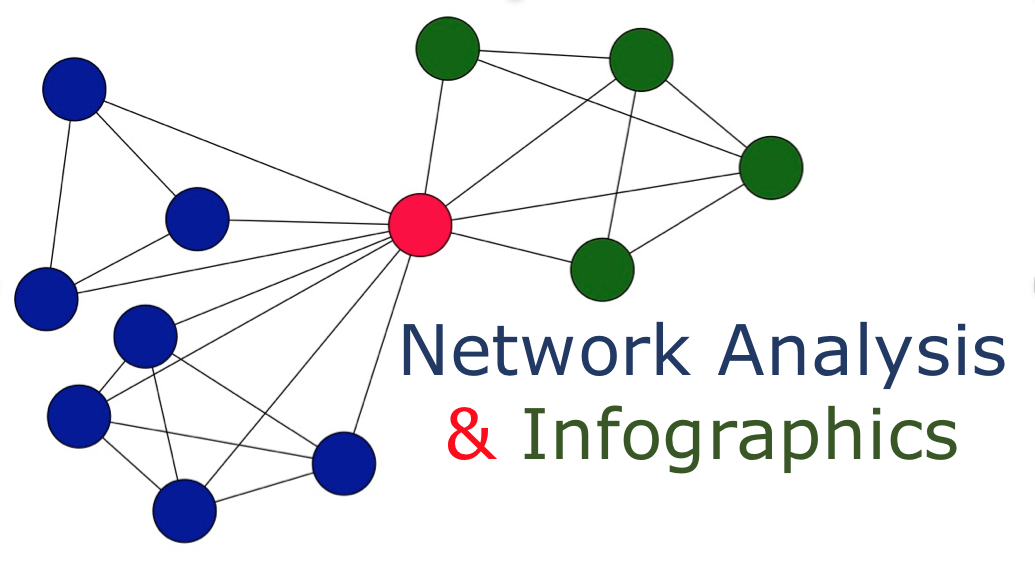
\includegraphics[width=2.5cm]{../_shared_pics/logo}

\medskip

\textit{{\color{dkgreen}{Week 5}}}\\
}


\date{} % Date, can be changed to a custom date

\begin{document}

\begin{frame}
\titlepage % Print the title page as the first slide

\begin{textblock*}{10pt}(0pt, 0.9\textheight)

\includegraphics[width=4cm]{../_shared_pics/SPRU.png}
\end{textblock*}

\end{frame}


%=======================================================
%	Learning outcomes
%=======================================================

\begin{frame}
\frametitle{Learning Outcomes}

\centering
\footnotesize
\begin{tabular}{lp{5.5cm}l}
\toprule
\multicolumn{2}{l}{\textbf{Learning outcome}} & \textbf{Assessment mode}\\
\hline
\\
1 & 
Explain the concept of network and list the main network indicators & 
ESS\\
\\
2 & 
Describe and apply the major techniques for the collection of network data and their statistical analysis & 
ESS, GPN + GWS\\
\\
\rowcolor{green!20}3 & 
Identify the main characteristics of networks by means of network measures  & 
ESS, GPN + GWS\\
\\
4 &
Employ network analysis techniques to produce network data-based infographics & 
GPN + GWS\\
\\
\bottomrule
\multicolumn{3}{l}{Note: ESS: Essay; GPN: Group Presentation; GWS: Group Written Submission}\\
\end{tabular}

\end{frame}

%------------------------------------------------





%=======================================================
% Network-level measures [recap]
%=======================================================
\section{Network-level measures [recap]}
%------------------------------------------------

\bgroup
\setbeamercolor{background canvas}{bg = navyblue}
\begin{frame}[plain]{}
\begin{center}
\color{white}{\Huge\insertsection}
\end{center}
\end{frame}
\egroup

%------------------------------------------------

\begin{frame}
\frametitle{\insertsection}

\footnotesize
\centering
\begin{tabular}{lp{7.5cm}}
\toprule
\textbf{Measure} & \textbf{Interpretation}\\
\hline
Diameter                        & Maximum time/resources for communication, transfer, ...\\
\\
APL                             & Average time/resources for communication, transfer, ...\\
\\
Density                         & Connectivity of a network \\
\\
Components                      & Presence of unconnected groups, bridging opportunities, ... \\
\\
Cutpoints and bridges           & Vulnerability/resilience of a network\\
\\
Point/Line connectivity         & Vulnerability/resilience of a network\\
\\
Cliques                         & Highly connected sub-groups, exclusion, ...\\
\\
Inclusiveness                   & Presence of unconnected nodes, exclusion, ... \\    
\\
Reachable pairs                 & Unconnected nodes or groups, bridging opportunities, ... \\
\\
Transitivity                    & Social interactions, `friends of my friends are my friends', ... \\

\bottomrule
\end{tabular}

\end{frame}

%------------------------------------------------






%=======================================================
%	Node-level measures
%=======================================================
\section{Node-level measures}
%------------------------------------------------

\bgroup
\setbeamercolor{background canvas}{bg = navyblue}
\begin{frame}[plain]{}
\begin{center}
\color{white}{\Huge\insertsection}
\end{center}
\end{frame}
\egroup

%------------------------------------------------

\begin{frame}
\frametitle{\insertsection}
\framesubtitle{Overview}

\begin{columns}

\column{.45\textwidth} 
\begin{enumerate}
\item Centrality
    \begin{itemize}
    \item Degree
    \item Closeness
    \item Betweenness
    \item Centralisation
    \item Bonacich's centrality
    \item Weighted centrality
    \end{itemize}
    
\medskip    

\item Brokerage
    \begin{itemize} 
    \item Brokerage roles
    \item Effective network size/efficiency
    \item Constraint
    \end{itemize}
\end{enumerate}


\column{.45\textwidth} 
\centering
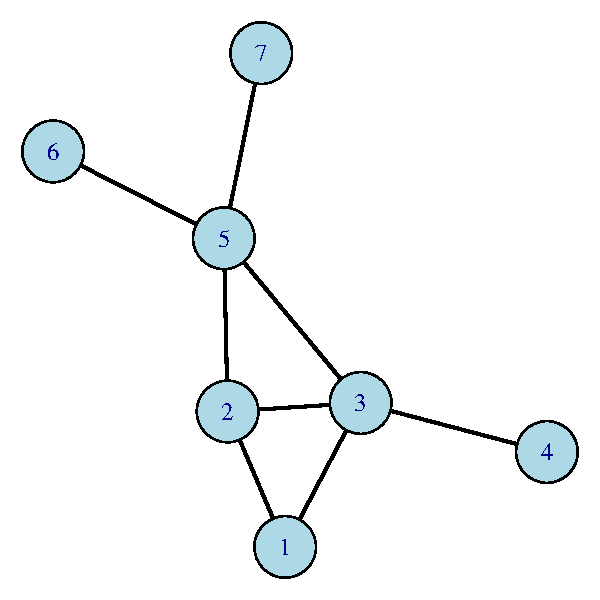
\includegraphics[width=5cm]{base}\\
\color{red}{\footnotesize Note: We will focus on\\ undirected and unweighted networks}

\end{columns}

\end{frame}

%------------------------------------------------

\begin{frame}
\frametitle{\insertsection}
\framesubtitle{Centrality}

{\color{blue}{Centrality}} measures provide an indication of the extent to which a node in a network is connected to the other nodes in the network \cite{Freeman1978}

\medskip

\begin{itemize}
\item Degree
\item Betweenness
\item Closeness
\end{itemize}

\end{frame}

%------------------------------------------------
\subsection{Degree centrality}
%------------------------------------------------

\begin{frame}
\frametitle{\insertsection}
\framesubtitle{\insertsubsection}

A node's {\color{blue}{degree}} is defined as the number of edges that are incident with it or the number of nodes that are adjacent to it 

\centering
\begin{equation*}
C_D(n_i) = \sum_{j=1, i \neq j}^{N-1}{x_{ij}}
\end{equation*}

\begin{equation*}
x_{ij} =\begin{cases}
    1, 	  & \text{if nodes $i$ and $j$ are linked}\\
    0, 	  & \text{otherwise}
  \end{cases}
\end{equation*}

\begin{itemize}
\item $C_D(n_i)$ can range from $0$ to $N-1$
\item If $C_D(n_i) = 0$, the node $n_i$ is called {\color{blue}{isolate}}
\item Degree helps to identify most {\color{blue}{active}}, {\color{blue}{popular}}, {\color{blue}{influential}} nodes
\end{itemize}

\end{frame}

%------------------------------------------------

\begin{frame}
\frametitle{\insertsection}
\framesubtitle{\insertsubsection}

\begin{columns}
	\column{.45\textwidth}
	\centering 
	\includegraphics<1>[width=5cm]{base}
	\includegraphics<2>[width=5cm]{degree}
	
	\onslide<2>\column{.45\textwidth}
	\small
	\renewcommand{\arraystretch}{1.5}
	\begin{table}
	\begin{tabular}{cc}
	\toprule
	$n_i$ & \textbf{$C_D(n_i) $}\\
	\hline
	1 & 2\\
	2 & 3\\
	3 & 4\\
	4 & 1\\
	5 & 4\\
	6 & 1\\
	7 & 1\\
	\bottomrule
	\end{tabular}
	\end{table}
\end{columns}

\end{frame}

%------------------------------------------------

\begin{frame}
\frametitle{\insertsection}
\framesubtitle{\insertsubsection}

\begin{columns}
\column{.45\textwidth} 
\begin{itemize}
\item Degree centrality is associated with the {\color{blue}{density}} of a network
\end{itemize}

\begin{equation*}
\Delta=\frac{\bar{C}_D}{N-1}
\end{equation*}

\begin{itemize}
\item $\bar{C}_D$ is the average degree
\end{itemize}

\column{.45\textwidth}

\centering
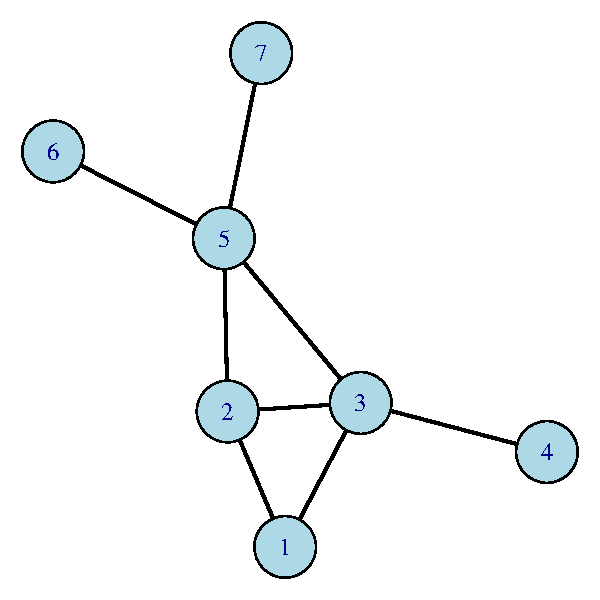
\includegraphics[width=5cm]{base}\\
\medskip

$\Delta=\frac{E}{\frac{N(N-1)}{2}}=\frac{8}{\frac{7(7-1)}{2}}=0.38$\\
\medskip

$\Delta=\frac{\bar{C}_D}{N-1}=\frac{\frac{(2+3+4+1+4+1+1)}{7}}{7-1}=0.38$

\end{columns}




\end{frame}

%------------------------------------------------

\begin{frame}[fragile]
\frametitle{\insertsection}
\framesubtitle{\insertsubsection \hspace{0.05cm} (distribution and scale-free networks)}

\begin{columns}[c]

\column{.5\textwidth}
\begin{minipage}[c][.5\textheight][c]{\linewidth}


Interactions between characters in The Godfather (1972) 
\begin{itemize}
\item $N = 42$
\item $E = 104$
\end{itemize}

\medskip
\medskip

\lstinputlisting[language = R, firstline = 39, lastline = 40]{handouts_script/L5_script_handouts.R}

\end{minipage}	   


\column{.5\textwidth}
\begin{minipage}[c][.5\textheight][c]{\linewidth}
\centering
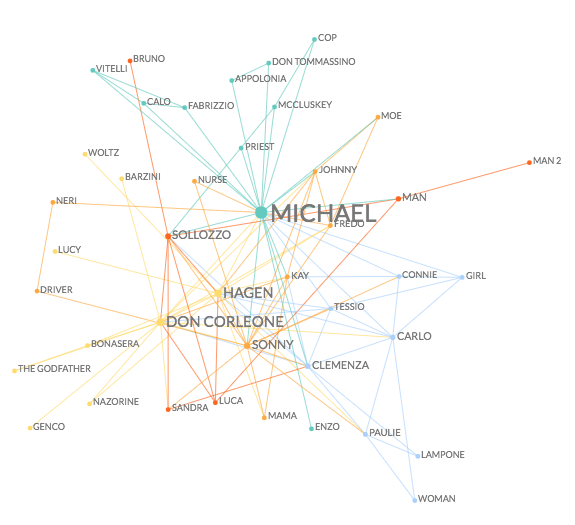
\includegraphics[width = \textwidth]{gf1}\\
\tiny Source: \url{http://moviegalaxies.com}
\end{minipage}

\end{columns}

\end{frame}
  

%------------------------------------------------

\begin{frame}
\frametitle{\insertsection}
\framesubtitle{\insertsubsection \hspace{0.05cm} (distribution and scale-free networks)}

\begin{columns}[c]

\column{.5\textwidth}
\centering
\tiny
\begin{tabular}{lc|lc}
\toprule
$n_i$ & $C_D(n_i)$ & $n_i$ & $C_D(n_i)$ \\
\hline
MICHAEL      & 25 & MAMA           & 3 \\
DON CORLEONE & 17 & MOE            & 3 \\
HAGEN        & 17 & VITELLI        & 3 \\
SONNY        & 15 & NERI           & 2 \\
CLEMENZA     & 11 & DRIVER         & 2 \\
SOLLOZZO     & 10 & APPOLONIA      & 2 \\
CARLO        & 9  & COP            & 2 \\
KAY          & 8  & DON TOMMASSINO & 2 \\
JOHNNY       & 7  & LAMPONE        & 2 \\
TESSIO       & 7  & NAZORINE       & 2 \\
PAULIE       & 6  & NURSE          & 2 \\
FREDO        & 6  & THE GODFATHER  & 2 \\
CONNIE       & 5  & WOMAN          & 2 \\
MAN          & 4  & BARZINI        & 1 \\
LUCA         & 4  & BRUNO          & 1 \\
GIRL         & 4  & ENZO           & 1 \\
SANDRA       & 4  & GENCO          & 1 \\
BONASERA     & 3  & LUCY           & 1 \\
MCCLUSKEY    & 3  & MAN 2          & 1 \\
CALO         & 3  & PRIEST         & 1 \\
FABRIZIO     & 3  & WOLTZ          & 1 \\
\bottomrule
\end{tabular}

\column{.5\textwidth}
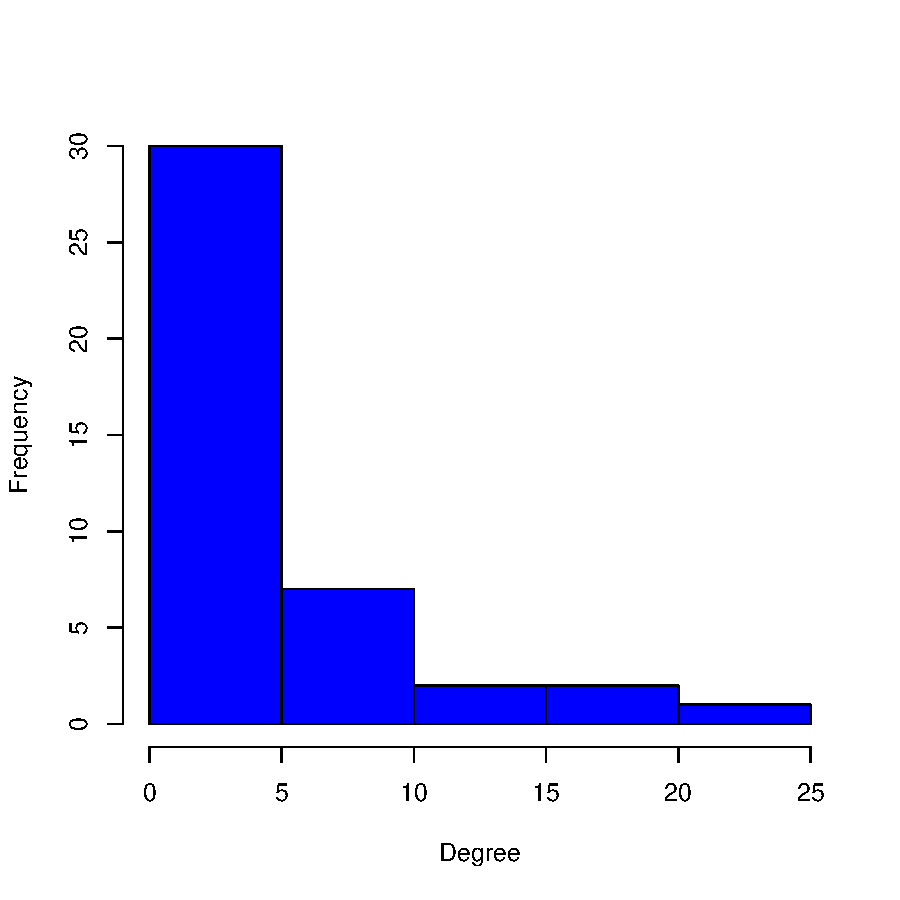
\includegraphics[width=5cm]{gf_dist}

\end{columns}


\begin{columns}[t]

\column{.5\textwidth} 
\lstinputlisting[language = R, firstline = 42, lastline = 43]{handouts_script/L5_script_handouts.R}

\column{.5\textwidth}
\lstinputlisting[language = R, firstline = 45, lastline = 51]{handouts_script/L5_script_handouts.R}

\end{columns}
 
\end{frame}

%------------------------------------------------

\begin{frame}[fragile]
\frametitle{\insertsection}
\framesubtitle{\insertsubsection \hspace{0.05cm} (distribution and scale-free networks)}

\begin{columns}[c]

\column{.5\textwidth}
\begin{minipage}[c][.5\textheight][c]{\linewidth}


{\color{blue}{Yeast data}} on protein-protein interaction in yeast
\begin{itemize}
\item $N = 2617$
\item $E = 11855$
\end{itemize}

\medskip
\medskip

\lstinputlisting[language = R, firstline = 14, lastline = 16]{handouts_script/L5_script_handouts.R}

\end{minipage}	   


\column{.5\textwidth}
\begin{minipage}[c][.5\textheight][c]{\linewidth}
\centering
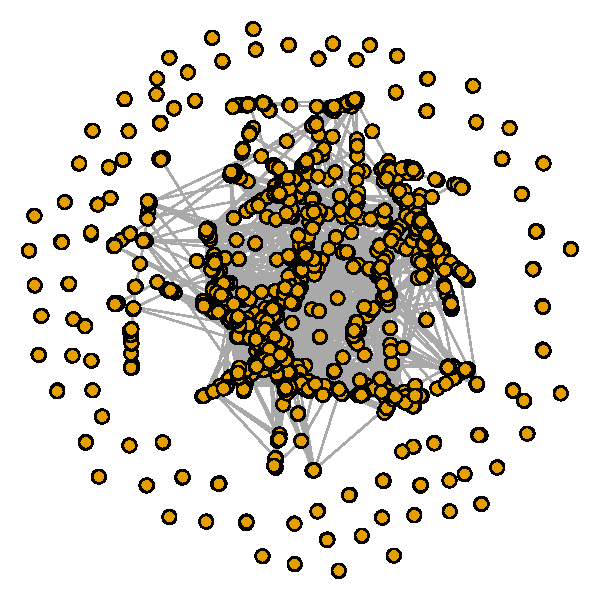
\includegraphics[width = \textwidth]{yeast_density}\\
\tiny Source: \cite{VonMering2002}
\end{minipage}

\end{columns}

\end{frame}
  

%------------------------------------------------

\begin{frame}
\frametitle{\insertsection}
\framesubtitle{\insertsubsection \hspace{0.05cm} (distribution and scale-free networks)}

\begin{columns}[c]

\column{.5\textwidth}
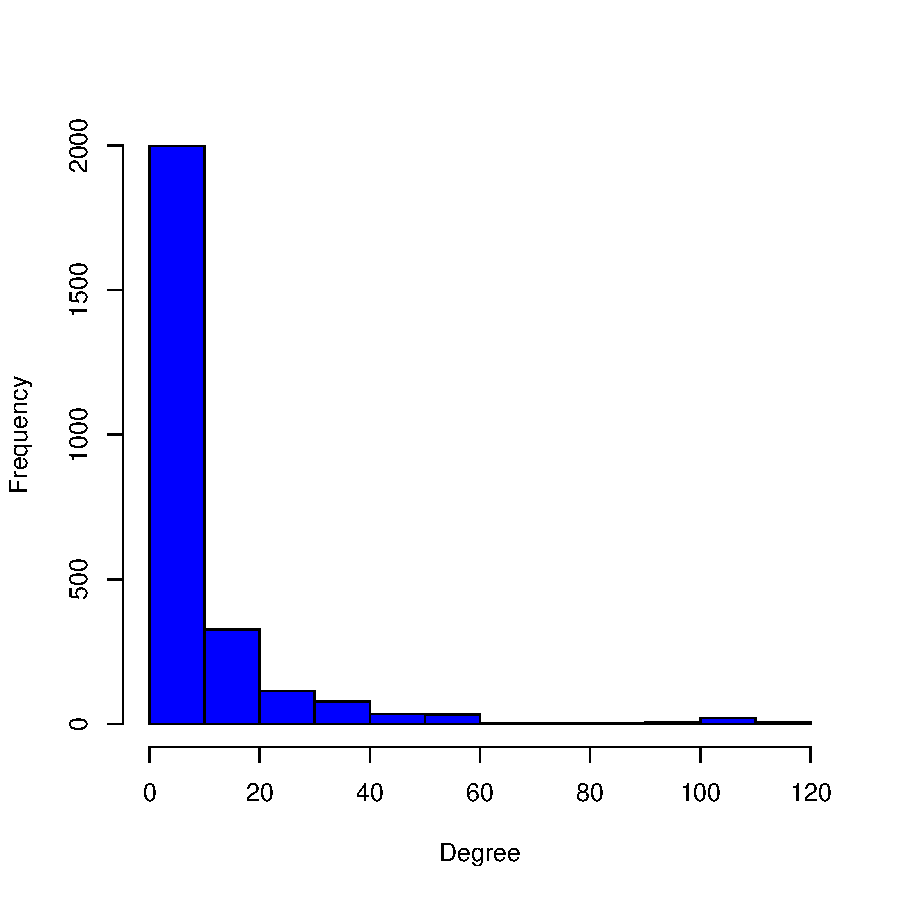
\includegraphics[width=5cm]{yeast1}

\column{.5\textwidth}
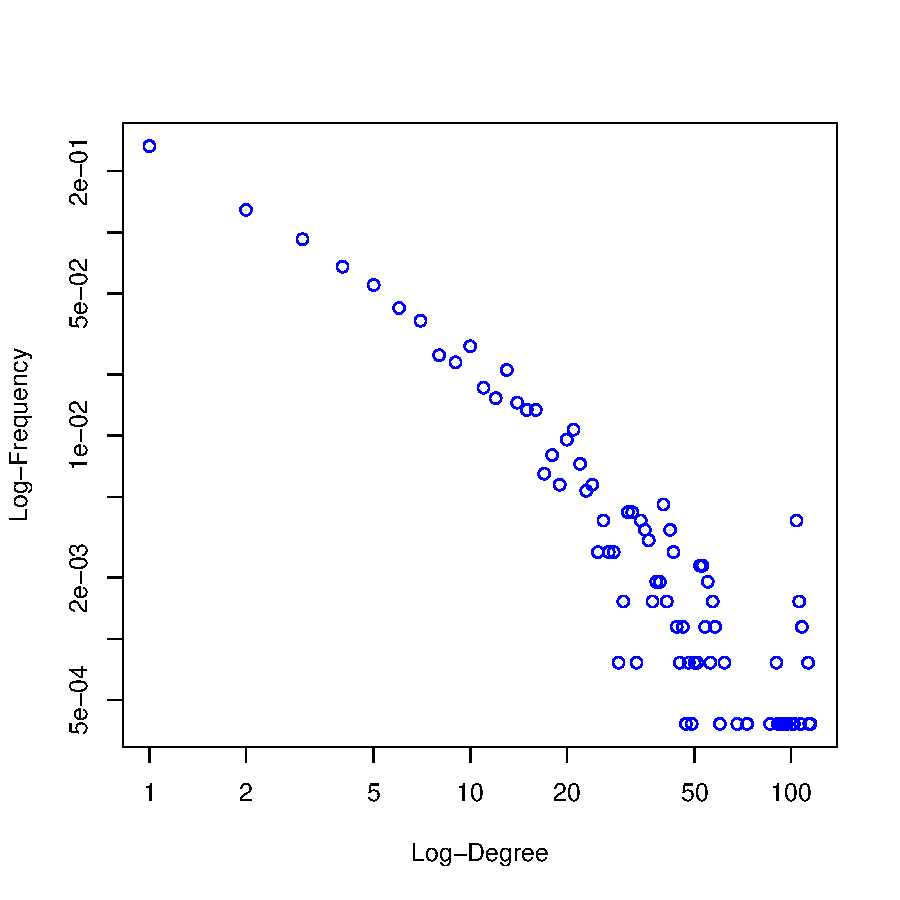
\includegraphics[width=5cm]{yeast2}

\end{columns}


\begin{columns}[t]

\column{.5\textwidth} 
\lstinputlisting[language=R, firstline=18, lastline=24]{handouts_script/L5_script_handouts.R}

\column{.5\textwidth}
\lstinputlisting[language=R, firstline=26, lastline=35]{handouts_script/L5_script_handouts.R}

\end{columns}
 
\end{frame}

%------------------------------------------------

\begin{frame}
\frametitle{\insertsection}
\framesubtitle{\insertsubsection \hspace{0.05cm} (distribution and scale-free networks)}

\begin{itemize}
	\item Large networks seems to self-organize into a {\color{blue}{scale-free state}}
	\item The probability that a node interacts with $k$ nodes follows a {\color{blue}{power law}}: $P(k) \sim k^{-\gamma}$
	\item $2<\gamma<3$, but also outside this range
	\item This feature is not predicted by current random network models
\end{itemize}

\medskip

\centering
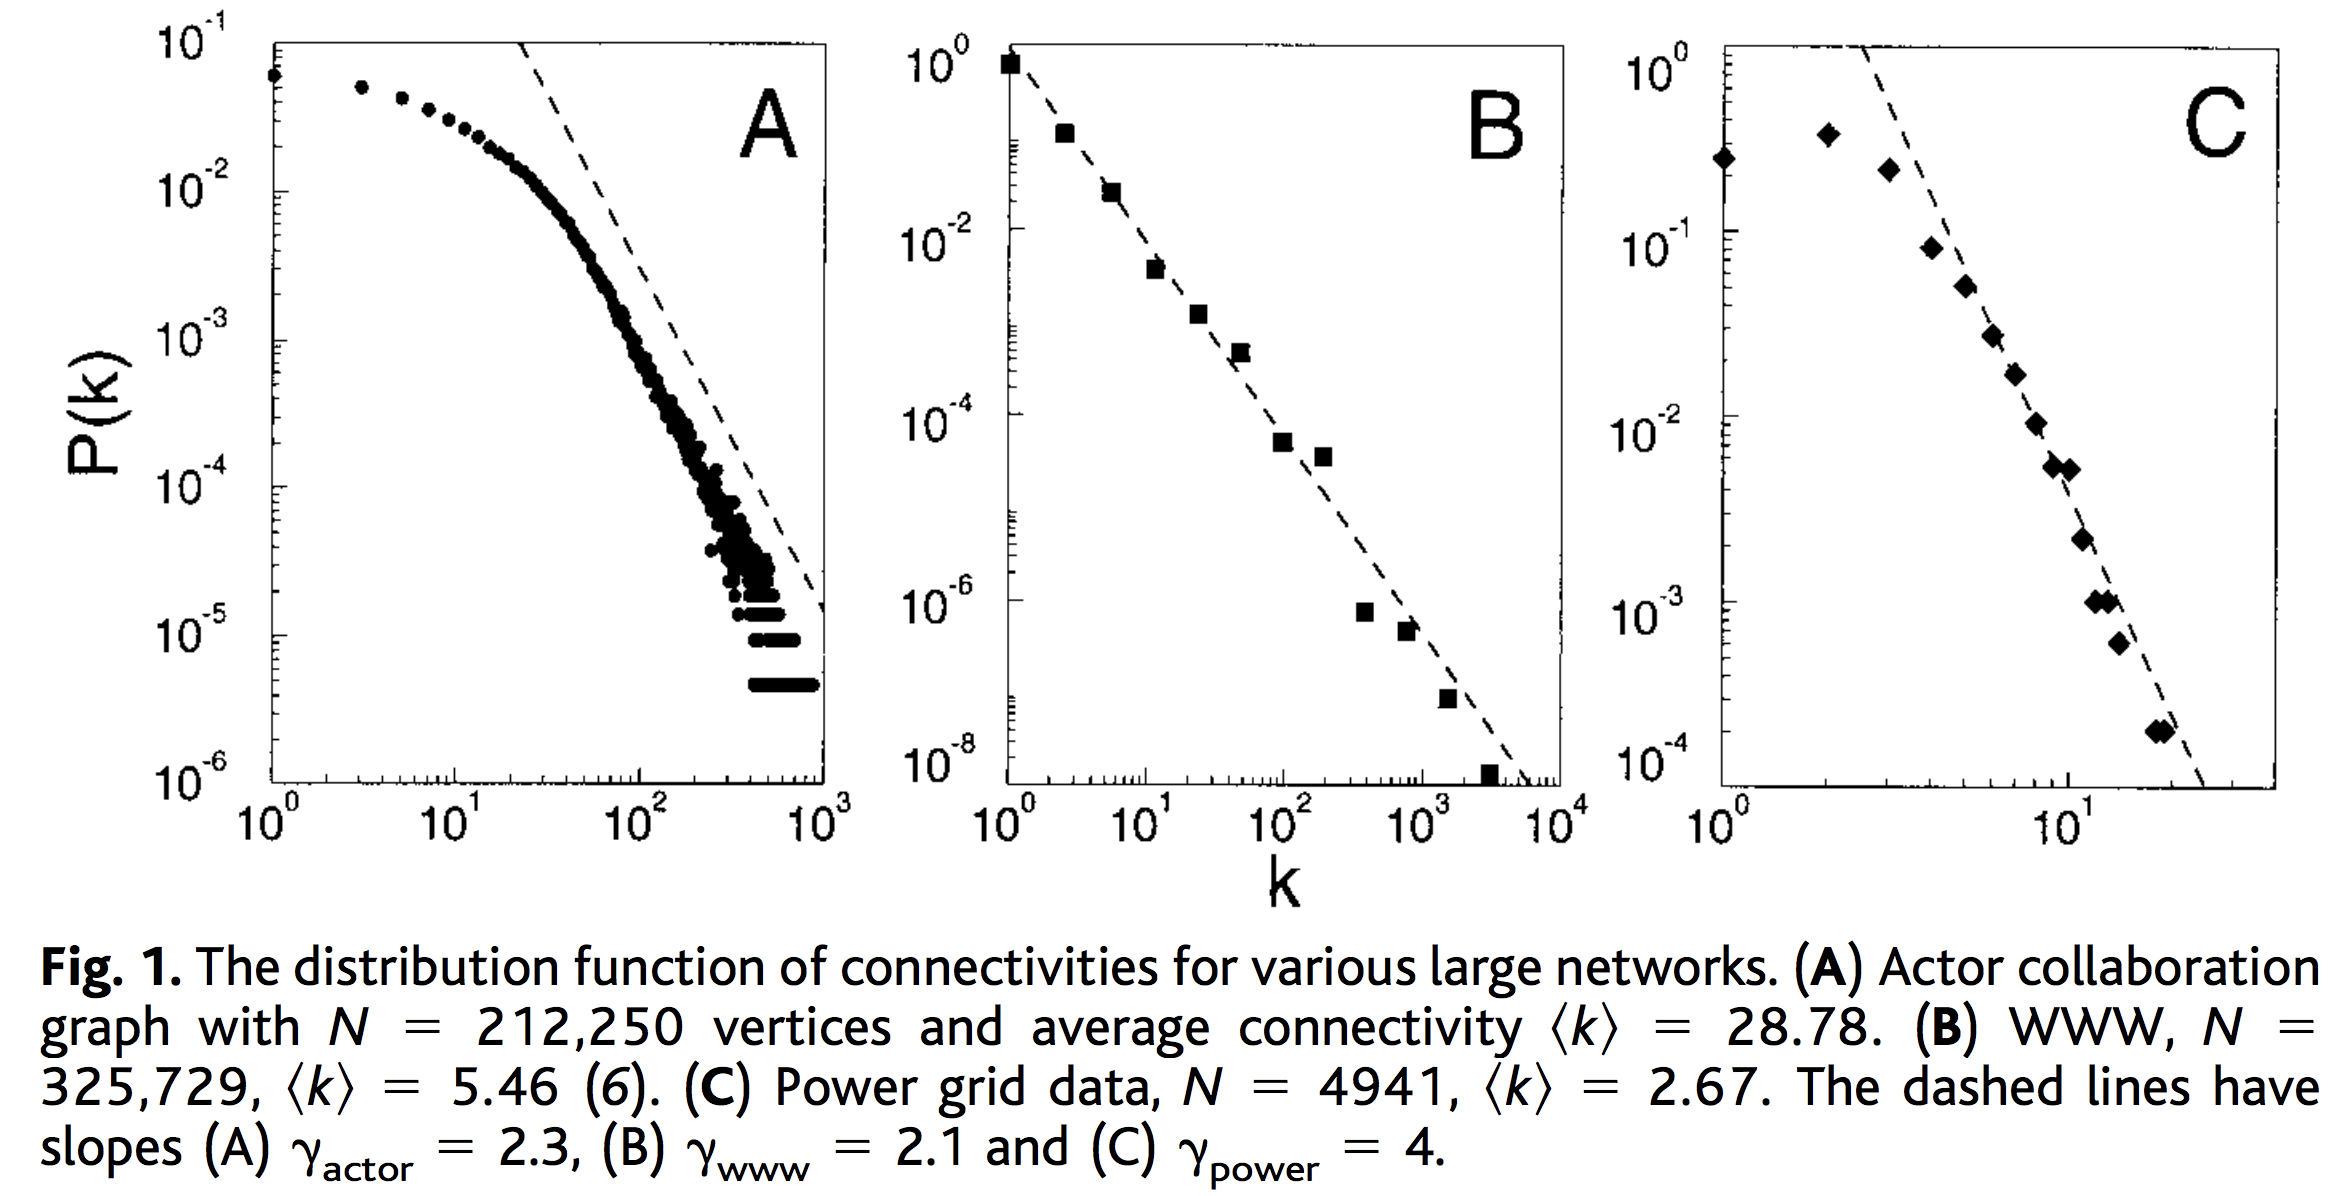
\includegraphics[width = 0.7\textwidth]{scale_free}\\
\tiny Source: \cite{Barabasi1999}
 
\end{frame}

%------------------------------------------------

\begin{frame}
\frametitle{\insertsection}
\framesubtitle{\insertsubsection \hspace{0.05cm} (distribution and scale-free networks)}

\centering
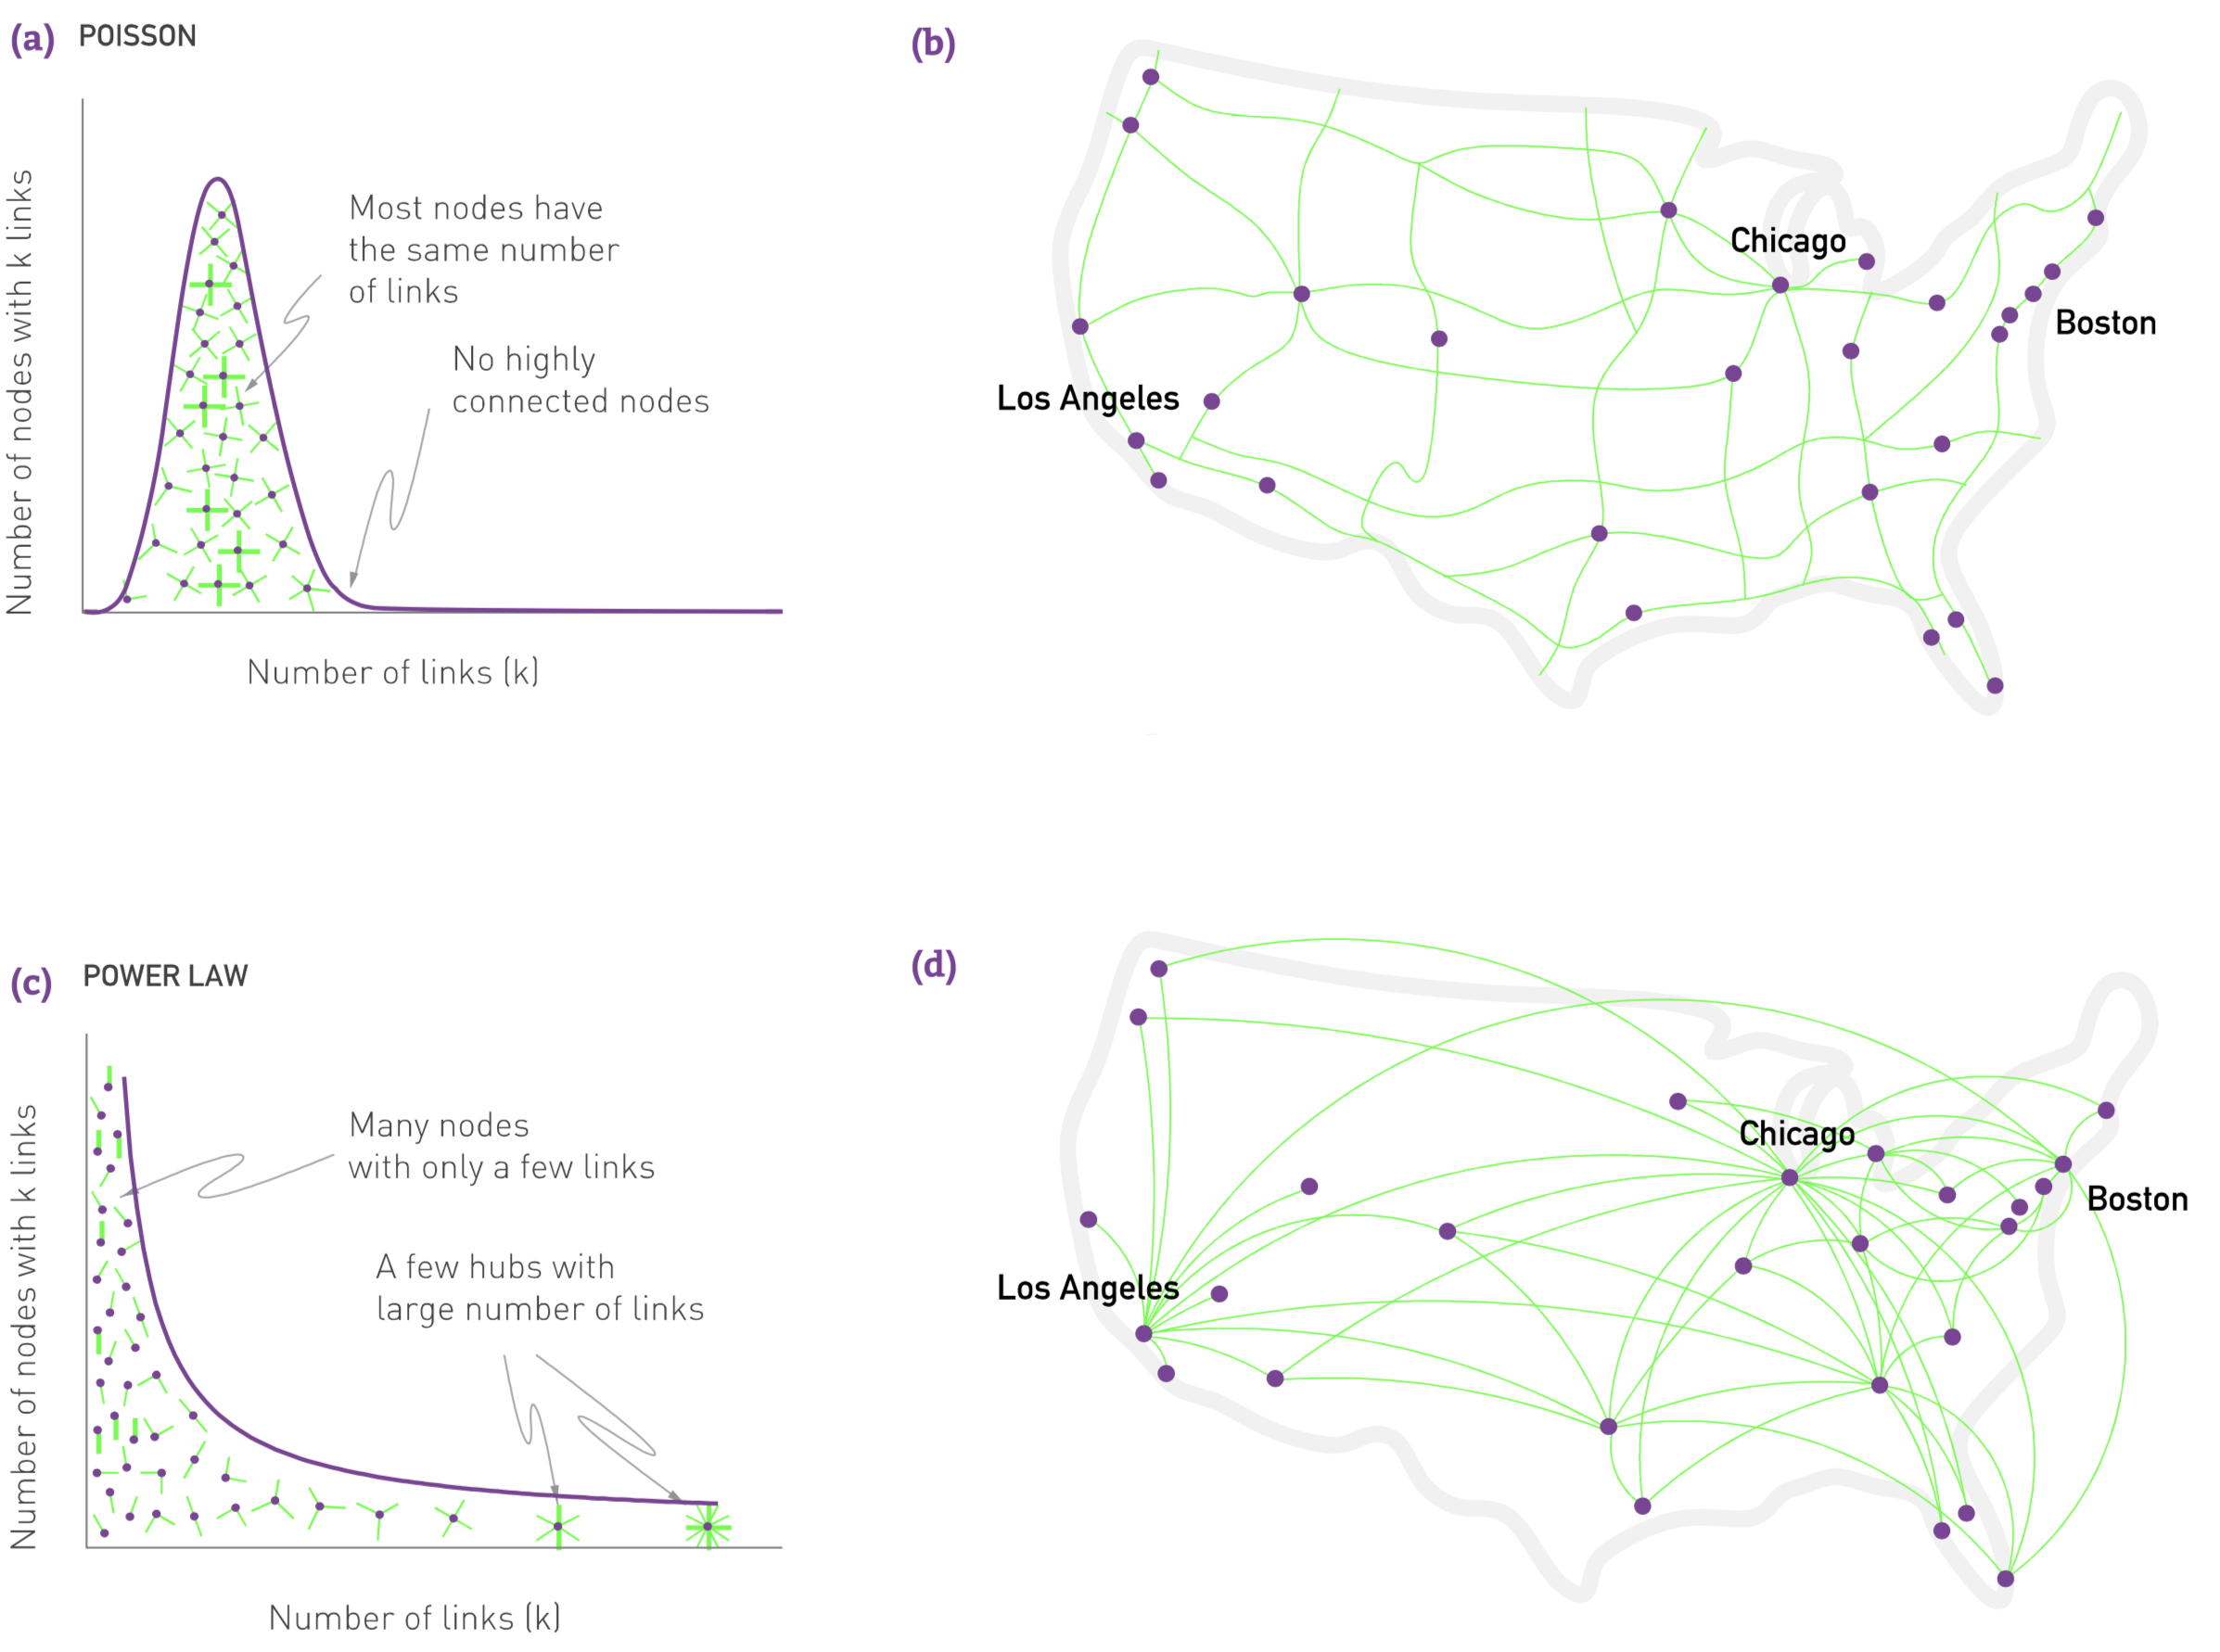
\includegraphics[height=0.8\textheight]{scale_free2}\\
\tiny{Source: Random networks (top, road connections) and scale-free networks (bottom, flight connections) \cite{Barabasi2016}}

\end{frame}


%Random networks: In other words nodes in a random network have comparable degrees and the average degree 〈k〉 serves as the “scale” of a random network.
%Scale-free networks: This means that when we randomly choose a node, we do not know what to expect: The selected node’s degree could be tiny or arbitrarily large. Hence networks with γ ‹ 3 do not have a meaningful internal scale, but are “scale-free”

%------------------------------------------------


\begin{frame}
\frametitle{\insertsection}
\framesubtitle{\insertsubsection \hspace{0.05cm} ($K$-core)}

\begin{columns}
\column{.45\textwidth} 

\begin{itemize}
\item A {\color{blue}{$k$-core}} is a subgraph in which each node has a degree of at least $k$
\item The $k$-core measure identifies nodes that are at the `core' of the network (especially if the network presents a core-periphery structure)
\end{itemize}

\column{.45\textwidth}
\centering
\includegraphics<1>[width=5cm]{base}
\includegraphics<2>[width=5cm]{kc1}
\includegraphics<3>[width=5cm]{kc2}

\end{columns}

\end{frame}

%------------------------------------------------

\begin{frame}
\frametitle{\insertsection}
\framesubtitle{\insertsubsection \hspace{0.05cm} ($K$-core)}

\centering
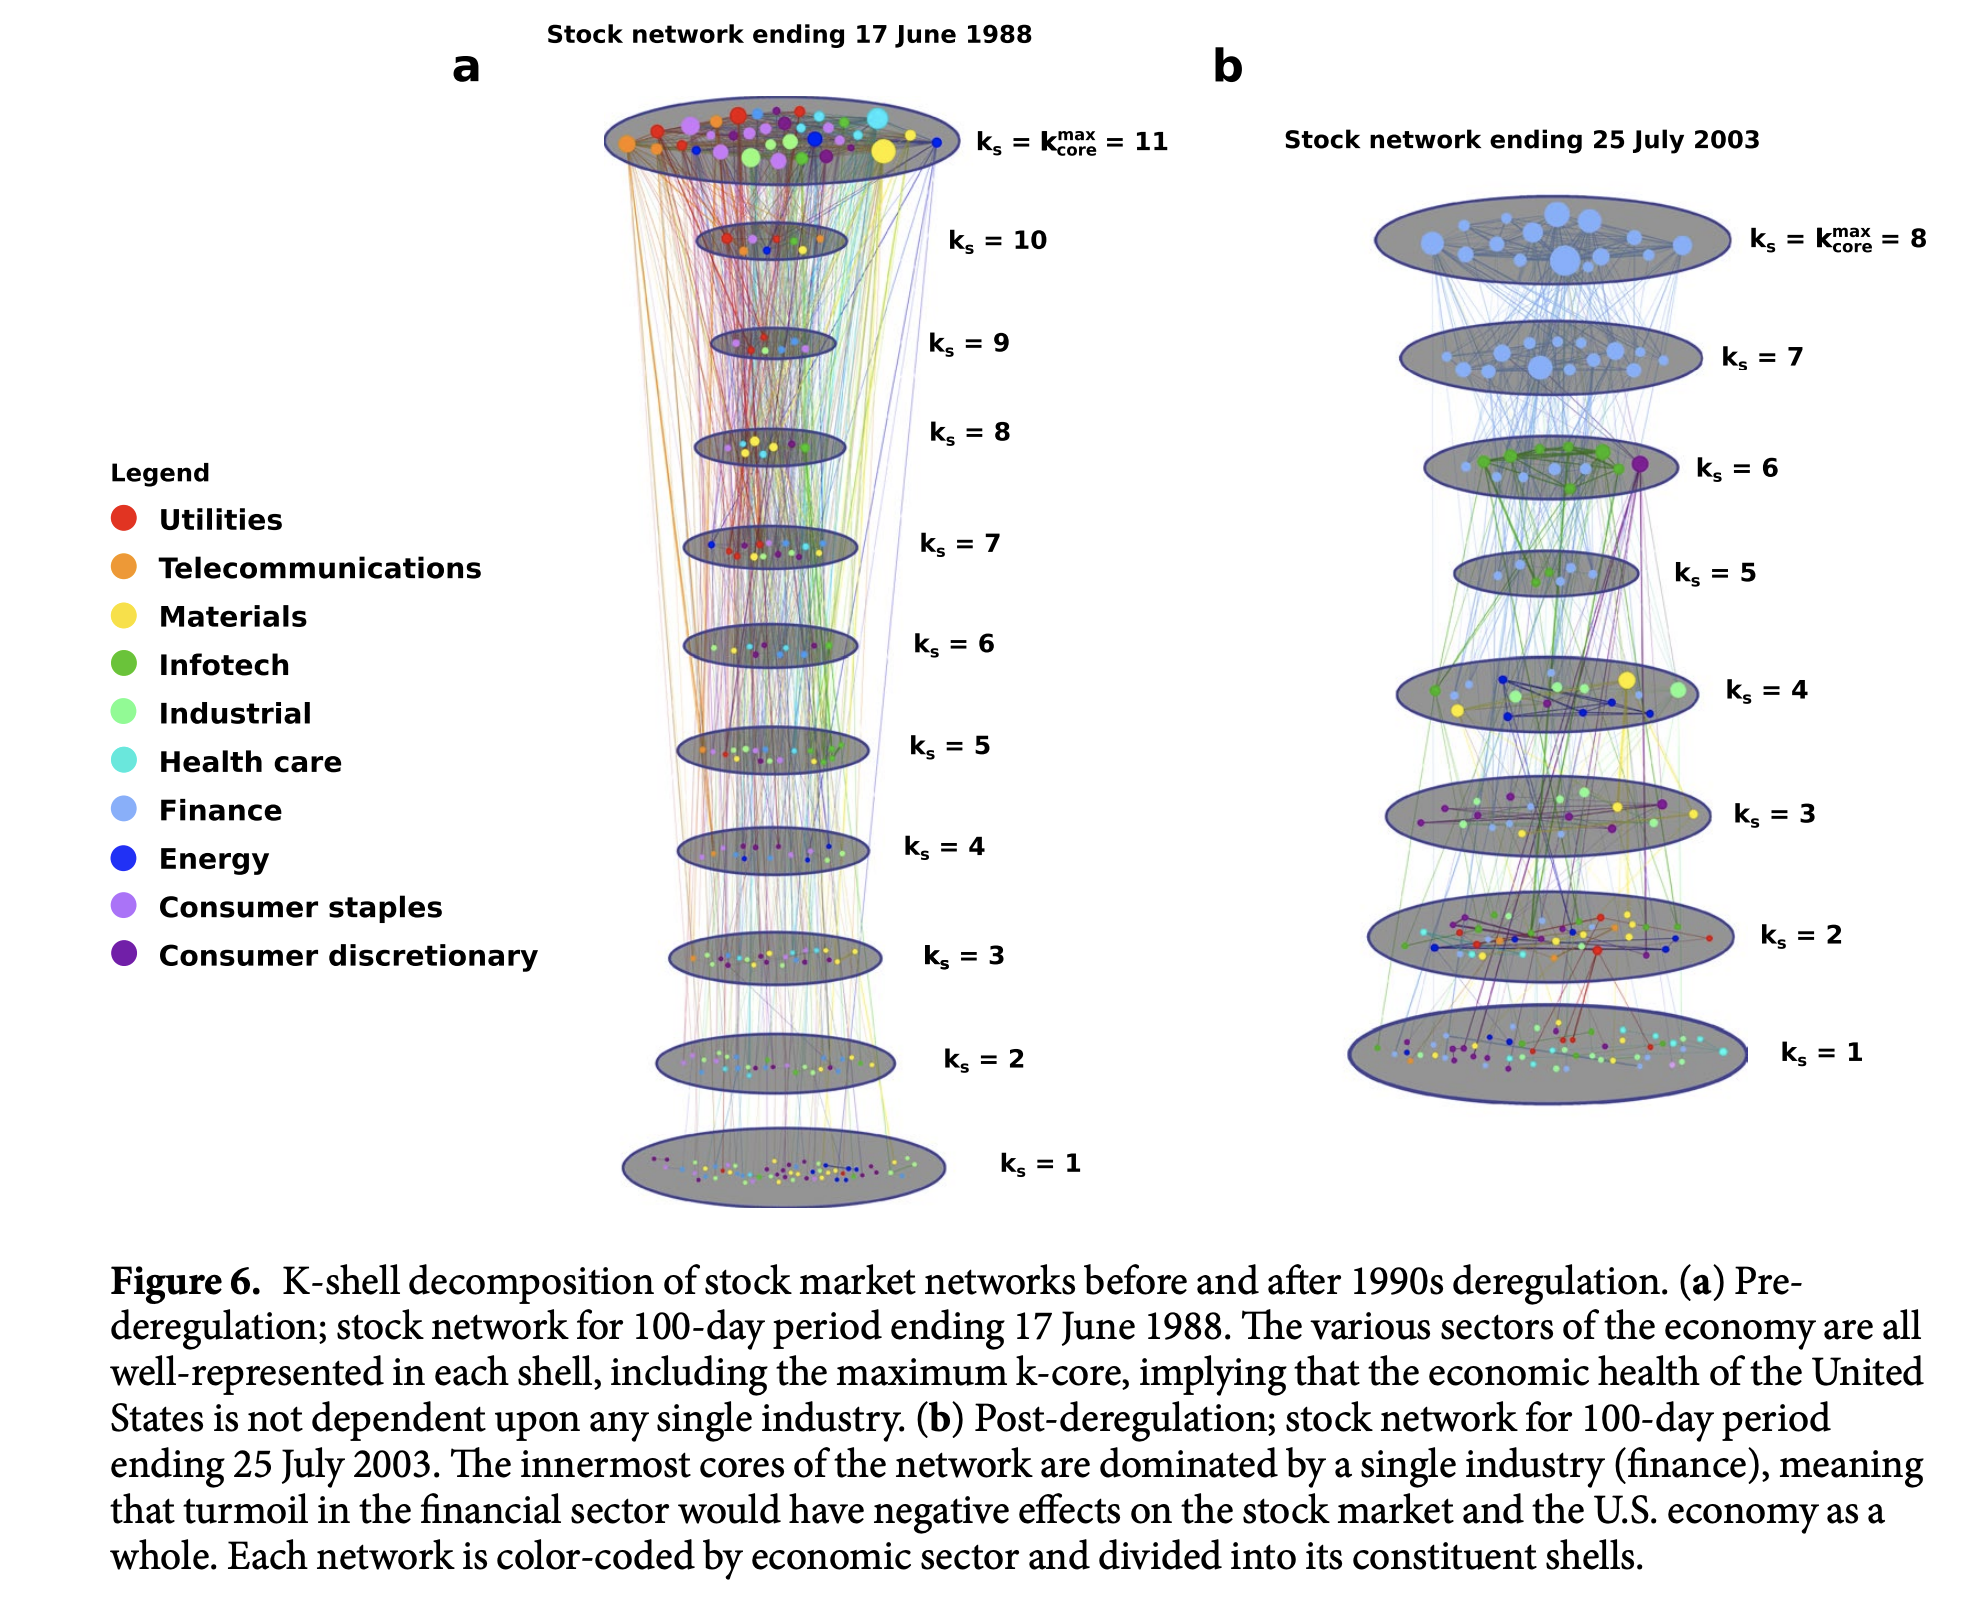
\includegraphics[width=9.5cm]{k_core_sector.png}\\
\tiny{Source: \cite{Burleson-Lesser2020}}

\end{frame}

% Regulation change and domination of one industry (finance)
% Interaction (links) between 500 S&P stocks are based on pairwise correlation of time series on stock log returns
% For the financial data, the matrices Cij (coorelation) can potentially show spurious correlations which arise not from similarities between the behaviours of two stocks, but from the similarity of each to a third stock. As an example, let us imagine three stocks A, B, and D. A and B do not behave in a similar fashion to each other, but they behave similarly (in two different ways) to D. Despite this, A and B would have a high value of correlation thus implying that they behave alike when they, in fact, do not. To find the true pairwise interactions Ji j, we turn to the Graphical Lasso (“Glasso”) algorithm of Friedman, Hastie, and Tibshirani
% Regulation  -- too big/core to fail (Clinton Adminsitration)
%Glass Steagall Act fu ridotto, banks started to merge

%------------------------------------------------
\subsection{Closeness centrality}
%------------------------------------------------

\begin{frame}
\frametitle{\insertsection}
\framesubtitle{\insertsubsection}


A node's {\color{blue}{closeness centrality}} is defined as the inverse of the sum of the geodesic distances of the node from all the nodes of the network


\centering
\begin{equation*}
C_C(n_i) = \frac{1}{\sum_{j=1, i \neq j}^{N-1} d(n_i, n_j)}
\end{equation*}

\begin{itemize}
\item \scalebox{1}{$d(n_i, n_j)$} is the geodesic distance between nodes $n_i$ and $n_j$
\item $C_C(n_i)$ can range from $0$ to $\frac{1}{N-1}$
	\begin{itemize}
	\item If $C_C(n_i) = 0$, one or more nodes are not reachable from $n_i$
	\item If $C_C(n_i) = \frac{1}{N-1}$, the node $n_i$ is adjacent to all other nodes
	\end{itemize}
\item Closeness helps to identify nodes that are {\color{blue}{close to most of the nodes}} in the network
\item Closeness is an indicator of {\color{blue}{speed of information dissemination}} (how long a node would take to reach the other nodes in the network)
\end{itemize}

\end{frame}

%------------------------------------------------

\begin{frame}
\frametitle{\insertsection}
\framesubtitle{\insertsubsection}

\begin{columns}
	\column{.45\textwidth}
	\centering 
	\includegraphics<1>[width=5cm]{base}
	\includegraphics<2>[width=5cm]{closeness}
	
	\onslide<2>\column{.45\textwidth}
	\small
          \renewcommand{\arraystretch}{1.5}
	\begin{table}
	\begin{tabular}{cc}
	\toprule
	$n_i$ & \textbf{$C_C(n_i) $}\\
	\hline
	1 & 0.08\\
	2 & 0.11\\
	3 & 0.12\\
	4 & 0.07\\
	5 & 0.12\\
	6 & 0.07\\
	7 & 0.07\\
	\bottomrule
	\end{tabular}
	\end{table}
\end{columns}

\end{frame}

%------------------------------------------------
\subsection{Betweenness centrality}
%------------------------------------------------

\begin{frame}
\frametitle{\insertsection}
\framesubtitle{\insertsubsection}


A node's {\color{blue}{betweenness centrality}} is the proportion of shortest paths between pairs of nodes that include the node

\centering
\begin{equation*}
C_B(n_i) = \sum_{j<k \text{ and } j,k \neq i}g_{jk}(n_i)/g_{jk}
\end{equation*}

\begin{itemize}
\item $g_{jk}(n_i)$ is the  number of shortest paths between nodes $n_j$ and $n_k$ that contain node $n_i$ (assumption of equally likely geodesic linkings)
\item $g_{jk}$ is the total number of shortest paths between nodes $n_j$ and $n_k$
\item $C_B(n_i)=0$ can range from $0$ to $\frac{(N-1)(N-2)}{2}$
	\begin{itemize}
	\item If $C_B(n_i)=0$, the node $n_i$ falls on no shortest paths
	\item If $C_B(n_i)=\frac{(N-1)(N-2)}{2}$, the node $n_i$ falls on all shortest paths
	\end{itemize}
\item Betweenness centrality helps to identify points where {\color{blue}{the network is likely break apart}} (this measure is related to the measure of cutpoints)
\item Betweenness centrality is an indicator of which nodes are more likely to be in the communication paths between other nodes: {\color{blue}{control}} and {\color{blue}{power}}

\end{itemize}

\end{frame}
%------------------------------------------------

\begin{frame}
\frametitle{\insertsection}
\framesubtitle{\insertsubsection}

\begin{columns}
	\column{.45\textwidth}
         \centering 
	\includegraphics<1>[width=5cm]{base}
	\includegraphics<2>[width=5cm]{betweenness}
	
	\onslide<2>\column{.45\textwidth}
	\small
	\renewcommand{\arraystretch}{1.5}
	\begin{table}
	\begin{tabular}{cc}
	\toprule
	$n_i$ & \textbf{$C_B(n_i) $}\\
	\hline
	1 & 0.00\\
	2 & 1.50\\
	3 & 6.50\\
	4 & 0.00\\
	5 & 9.00\\
	6 & 0.00\\
	7 & 0.00\\
	\bottomrule
	\end{tabular}
	\end{table}
\end{columns}

\end{frame}
%------------------------------------------------
\subsection{Centrality standardisation}
%------------------------------------------------

\begin{frame}
\frametitle{\insertsection}
\framesubtitle{\insertsubsection}

\begin{itemize}
\item Centrality measures are dependent on the {\color{blue}{size of a network}}
\item {\color{blue}{Comparison}} between network of different size can be misleading
\item The {\color{blue}{standard normalisation}} approach account for the size of the network
\end{itemize}

\begin{equation*}
C_D^{'}(n_i) = \frac{C_D(n_i) }{N-1}
\end{equation*}

\begin{equation*}
C_C^{'}(n_i) = (N-1) C_C(n_i)
\end{equation*}

\begin{equation*}
C_B^{'}(n_i) = \frac{C_B(n_i)}{(N-1)(N-2)/2}
\end{equation*}

\begin{itemize}
\onslide<2>{\item {\color{red}{This does not completely address the size effect issue}} (e.g.\ friendship network of 1000 nodes vs.\ friendship network of 10 nodes)}
\end{itemize}

\end{frame}

%------------------------------------------------

\begin{frame}
\frametitle{\insertsection}
\framesubtitle{\insertsubsection \hspace{0.05cm} (degree)}

\begin{columns}
	\column{.45\textwidth}
	\centering 
	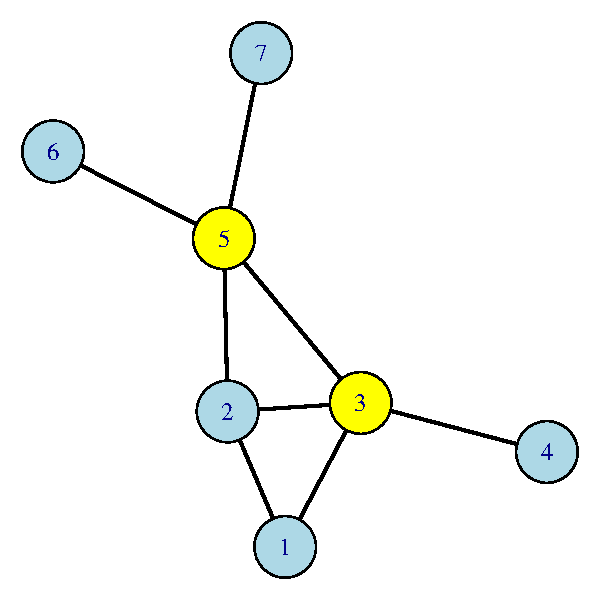
\includegraphics[width=5cm]{degree}
	
	\column{.45\textwidth}
	\small
	\renewcommand{\arraystretch}{1.5}
	\begin{table}
	\begin{tabular}{ccc}
		\toprule
	$n_i$ & $C_D(n_i) $ & $C_D^{'}(n_i)$\\
	\hline
	1 & 2 & $\frac{2}{7-1}=0.33$\\
	2 & 3 & $\frac{3}{7-1}=0.50$\\
	3 & 4 & $\frac{4}{7-1}=0.67$\\
	4 & 1 & $\frac{1}{7-1}=0.17$\\
	5 & 4 & $\frac{4}{7-1}=0.67$\\
	6 & 1 & $\frac{1}{7-1}=0.17$\\
	7 & 1 & $\frac{1}{7-1}=0.17$\\
	\bottomrule
	\end{tabular}
	\end{table}
	
\end{columns}
\end{frame}

%------------------------------------------------

\begin{frame}
\frametitle{\insertsection}
\framesubtitle{\insertsubsection \hspace{0.05cm} (closeness)}

\begin{columns}
	\column{.45\textwidth}
	\centering 
	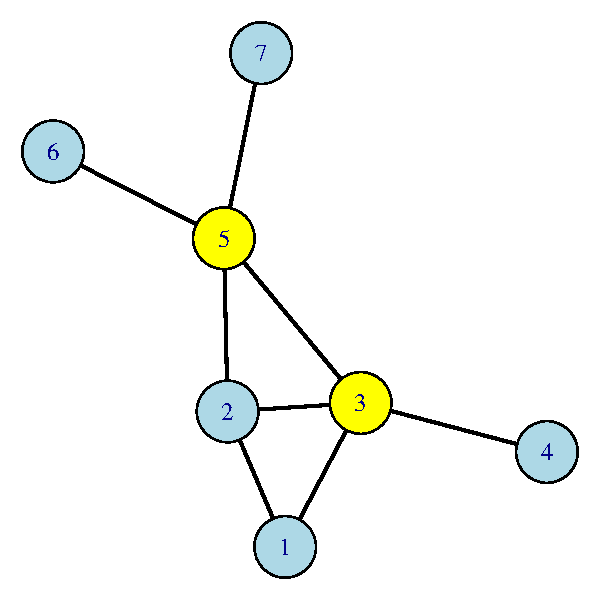
\includegraphics[width=5cm]{closeness}
	
	\column{.45\textwidth}
	\small
	\renewcommand{\arraystretch}{1.5}
	\begin{table}
	\begin{tabular}{ccc}
		\toprule
	$n_i$ & $C_C(n_i) $ & $C_C^{'}(n_i)$\\
	\hline
	1 & 0.08 & $(7-1)*0.08=0.50$\\
	2 & 0.11 & $(7-1)*0.11=0.67$\\
	3 & 0.12 & $(7-1)*0.12=0.75$\\
	4 & 0.07 & $(7-1)*0.07=0.46$\\
	5 & 0.12 & $(7-1)*0.12=0.75$\\
	6 & 0.07 & $(7-1)*0.07=0.46$\\
	7 & 0.07 & $(7-1)*0.07=0.46$\\
	\bottomrule
	\end{tabular}
	\end{table}
\end{columns}
\end{frame}

%------------------------------------------------

\begin{frame}
\frametitle{\insertsection}
\framesubtitle{\insertsubsection \hspace{0.05cm} (betweenness)}


\begin{columns}
	\column{.45\textwidth}
	\centering  
	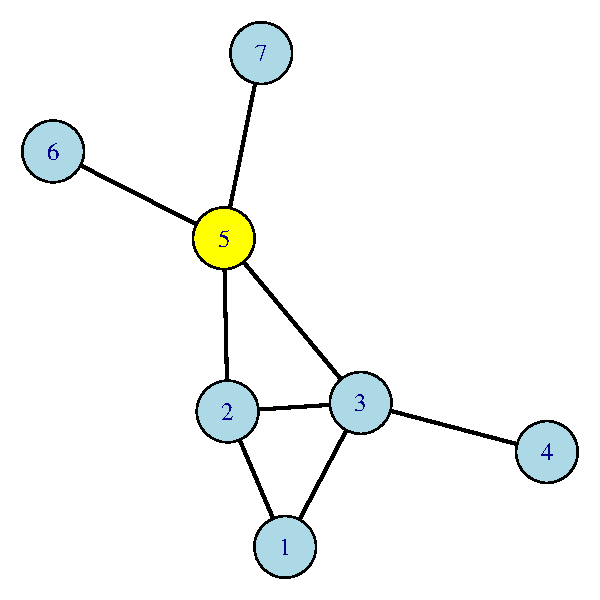
\includegraphics[width=5cm]{betweenness}
	
	\column{.45\textwidth}
	\small
	\renewcommand{\arraystretch}{1.5}
	\begin{table}
	\begin{tabular}{ccc}
		\toprule
	$n_i$ & $C_B(n_i) $ & $C_B^{'}(n_i)$\\
	\hline
	1 & 0.00 & $\frac{0.00}{\frac{(7-1)*(7-2)}{2}}=0.00$\\
	2 & 1.50 & $\frac{1.50}{\frac{(7-1)*(7-2)}{2}}=0.10$\\
	3 & 6.50 & $\frac{6.50}{\frac{(7-1)*(7-2)}{2}}=0.43$\\
	4 & 0.00 & $\frac{0.00}{\frac{(7-1)*(7-2)}{2}}=0.00$\\
	5 & 9.00 & $\frac{9.00}{\frac{(7-1)*(7-2)}{2}}=0.60$\\
	6 & 0.00 & $\frac{0.00}{\frac{(7-1)*(7-2)}{2}}=0.00$\\
	7 & 0.00 & $\frac{0.00}{\frac{(7-1)*(7-2)}{2}}=0.00$\\
	\bottomrule
	\end{tabular}
	\end{table}
\end{columns}
\end{frame}

%------------------------------------------------
\subsection{Centrality comparison}
%------------------------------------------------

\begin{frame}
\frametitle{\insertsection}
\framesubtitle{\insertsubsection}


\begin{columns}
	\column{.45\textwidth}
	\centering  
	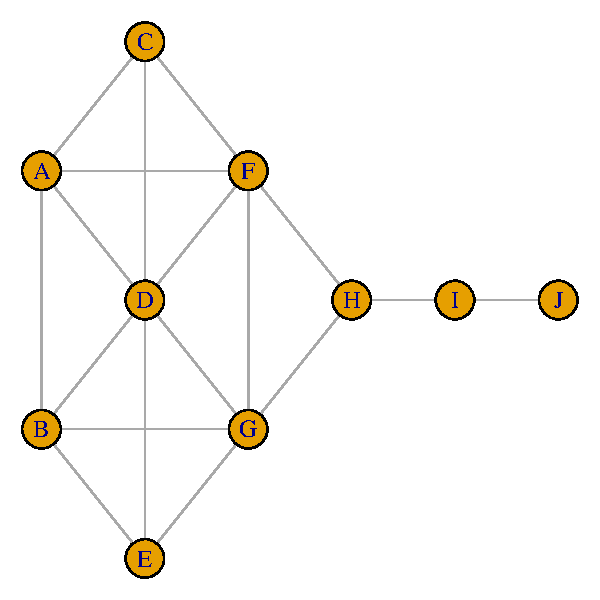
\includegraphics[width=5cm]{kite}\\
	\tiny Source: Krackhardt's fictionary social network (igraphdata) \cite{Krackhardt1990a}\\
	
	\column{.45\textwidth}
	\footnotesize
	\renewcommand{\arraystretch}{1.5}
	\begin{table}
	\begin{tabular}{cccc}
       \toprule
        $n_i$ & $C_D(n_i)$ & $C_C(n_i)$ & $C_B(n_i)$\\
        \hline
        A & 4 & 0.06 & 0.83\\
        B & 4 & 0.06 & 0.83\\
        C & 3 & 0.06 & 0.00\\
        D & \cellcolor{yellow}6 & \cellcolor{orange!50}0.07 & 3.67\\
        E & 3 & 0.06 & 0.00\\
        F & \cellcolor{yellow}5 & \cellcolor{orange!50}0.07 & \cellcolor{green!50}8.33\\
        G & \cellcolor{yellow}5 & \cellcolor{orange!50}0.07 & \cellcolor{green!50}8.33\\
        H & 3 & \cellcolor{orange!50}0.07 & \cellcolor{green!50}14.00\\
        I & 2 & 0.05 & 8.00\\
        J & 1 & 0.03 & 0.00\\
	\bottomrule
	\end{tabular}
	\end{table}
\end{columns}
\end{frame}

%------------------------------------------------ 

\begin{frame}
\frametitle{\insertsection}
\framesubtitle{Centralization}

\begin{itemize}
\item The {\color{blue}{distribution of centrality}} can provide some indication of the extent to which a network is centralized
\item \cite{Freeman1978} proposed the below measure of {\color{blue}{centralization}}
\end{itemize}

\begin{equation*}
C_X = \frac{\sum_{i=1}^{N}[C_X(p^*)-C_X(n_i)]}{max\sum_{i=1}^{N}[C_X(p^*)-C_X(n_i)]}
\end{equation*}

\begin{itemize}
\item $C_X(n_i)$, value of centrality for node $i$
\item $C_X(p^*)$, largest value of centrality 
\item The denominator can be theoretically calculated
	\begin{itemize}
	\item Degree: $(N-1)(N-2)$
	\item Closeness: $(N^2-3N+2)/(2N-2)$
	\item Betweenness: $N^3-4N^2+5N-2$
	\end{itemize}
\end{itemize}

\end{frame}

%------------------------------------------------

\begin{frame}
\frametitle{\insertsection}
\framesubtitle{Centralization}


\begin{columns}
	\column{.45\textwidth}
	\centering  
	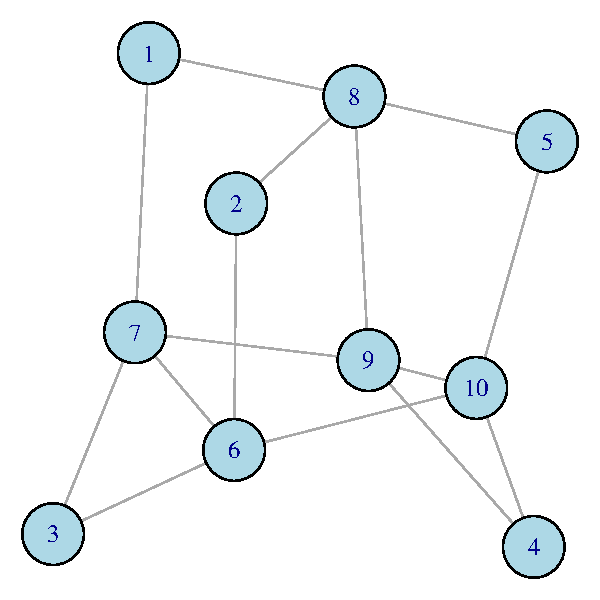
\includegraphics[width=5cm]{centralization1.pdf}
	
	\begin{itemize}
	\item $C_D = 0.14$
	\item $C_C = 0.25$
	\item $C_B = 0.14$
	\end{itemize}

	
	\column{.45\textwidth}
	\centering  
	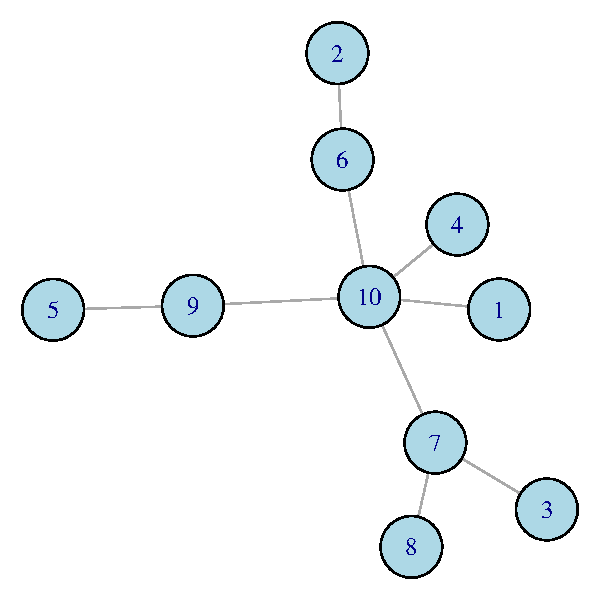
\includegraphics[width=5cm]{centralization2.pdf}
	
	\begin{itemize}
	\item $C_D = 0.44$
	\item $C_C = 0.52$
	\item $C_B = 0.72$
	\end{itemize}
	
\end{columns}
\end{frame}

%------------------------------------------------ 



%------------------------------------------------
\subsection{Bonacich's centrality}
%------------------------------------------------

\begin{frame}
\frametitle{\insertsection}
\framesubtitle{Bonacich's centrality}

\begin{itemize}
	\item The vector of {\color{blue}{Bonacich's centrality (power centrality)}} scores is defined as \cite{Bonacich1987}:
\end{itemize}

\centering
\begin{equation*}
c_i(\alpha,\beta) = \sum_{j}(\alpha+\beta c_j)A_{ij}
\end{equation*}

\begin{itemize}
	\item $\alpha$ is a scaling vector used to normalise the centrality values (convergence)
	\item $\beta$ is a parameter that defines the weight of the centrality of $i$'s neighbour nodes
	\item $A$ is the adjacency matrix
\end{itemize}

\end{frame}
%------------------------------------------------

\begin{frame}
\frametitle{\insertsection}
\framesubtitle{Bonacich's centrality}

\begin{itemize}
	\item $\beta = 0$: a node's centrality does not depend from the centrality of other nodes
	\item $\beta > 0$: a node's centrality {\color{blue}{positively}} depends on the centrality of its neighbours
	\item $\beta < 0$: a node's centrality {\color{blue}{negatively}} depends on the centrality of its neighbours (e.g.\  being link to a central node reduces the node's centrality or influence)
	\item Heuristic: $\beta$ at $3/4$ of the reciprocal of the largest eigenvalue of the adjacency matrix  
\end{itemize}

\end{frame}
%------------------------------------------------

\begin{frame}
\frametitle{\insertsection}
\framesubtitle{Bonacich's centrality (example)}

\centering
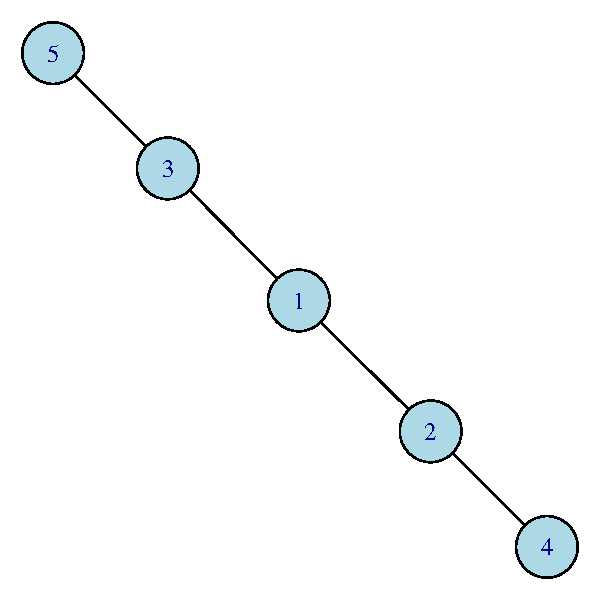
\includegraphics[width=5cm]{bonacich}
	
\small
\begin{table}
\begin{tabular}{cccccc}
\toprule
$n_i$ 	& \multicolumn{5}{c}{\textbf{$c_i(\alpha,\beta)$}}\\
\cline{2-6}
& 
$\beta = -0.50$ &
$\beta = -0.25$ &
$\beta =  0.00$ &
$\beta =  0.25$ &
$\beta =  0.50$\\

\hline
1 & 0.00 & 1.04 & \cellcolor{green!50}1.20 & \cellcolor{green!50}1.25 & \cellcolor{green!50}1.28 \\
2 & \cellcolor{green!50}1.58 & \cellcolor{green!50}1.30 & \cellcolor{green!50}1.20 & 1.15 & 1.12 \\
3 & \cellcolor{green!50}1.58 & \cellcolor{green!50}1.30 & \cellcolor{green!50}1.20 & 1.15 & 1.12 \\
4 & 0.00 & 0.52 & 0.60 & 0.63 & 0.64 \\
5 & 0.00 & 0.52 & 0.60 & 0.63 & 0.64 \\
\bottomrule
\end{tabular}
\end{table}

\end{frame}

%------------------------------------------------

\begin{frame}
\frametitle{\insertsection}
\framesubtitle{Bonacich's centrality (example)}

\centering  
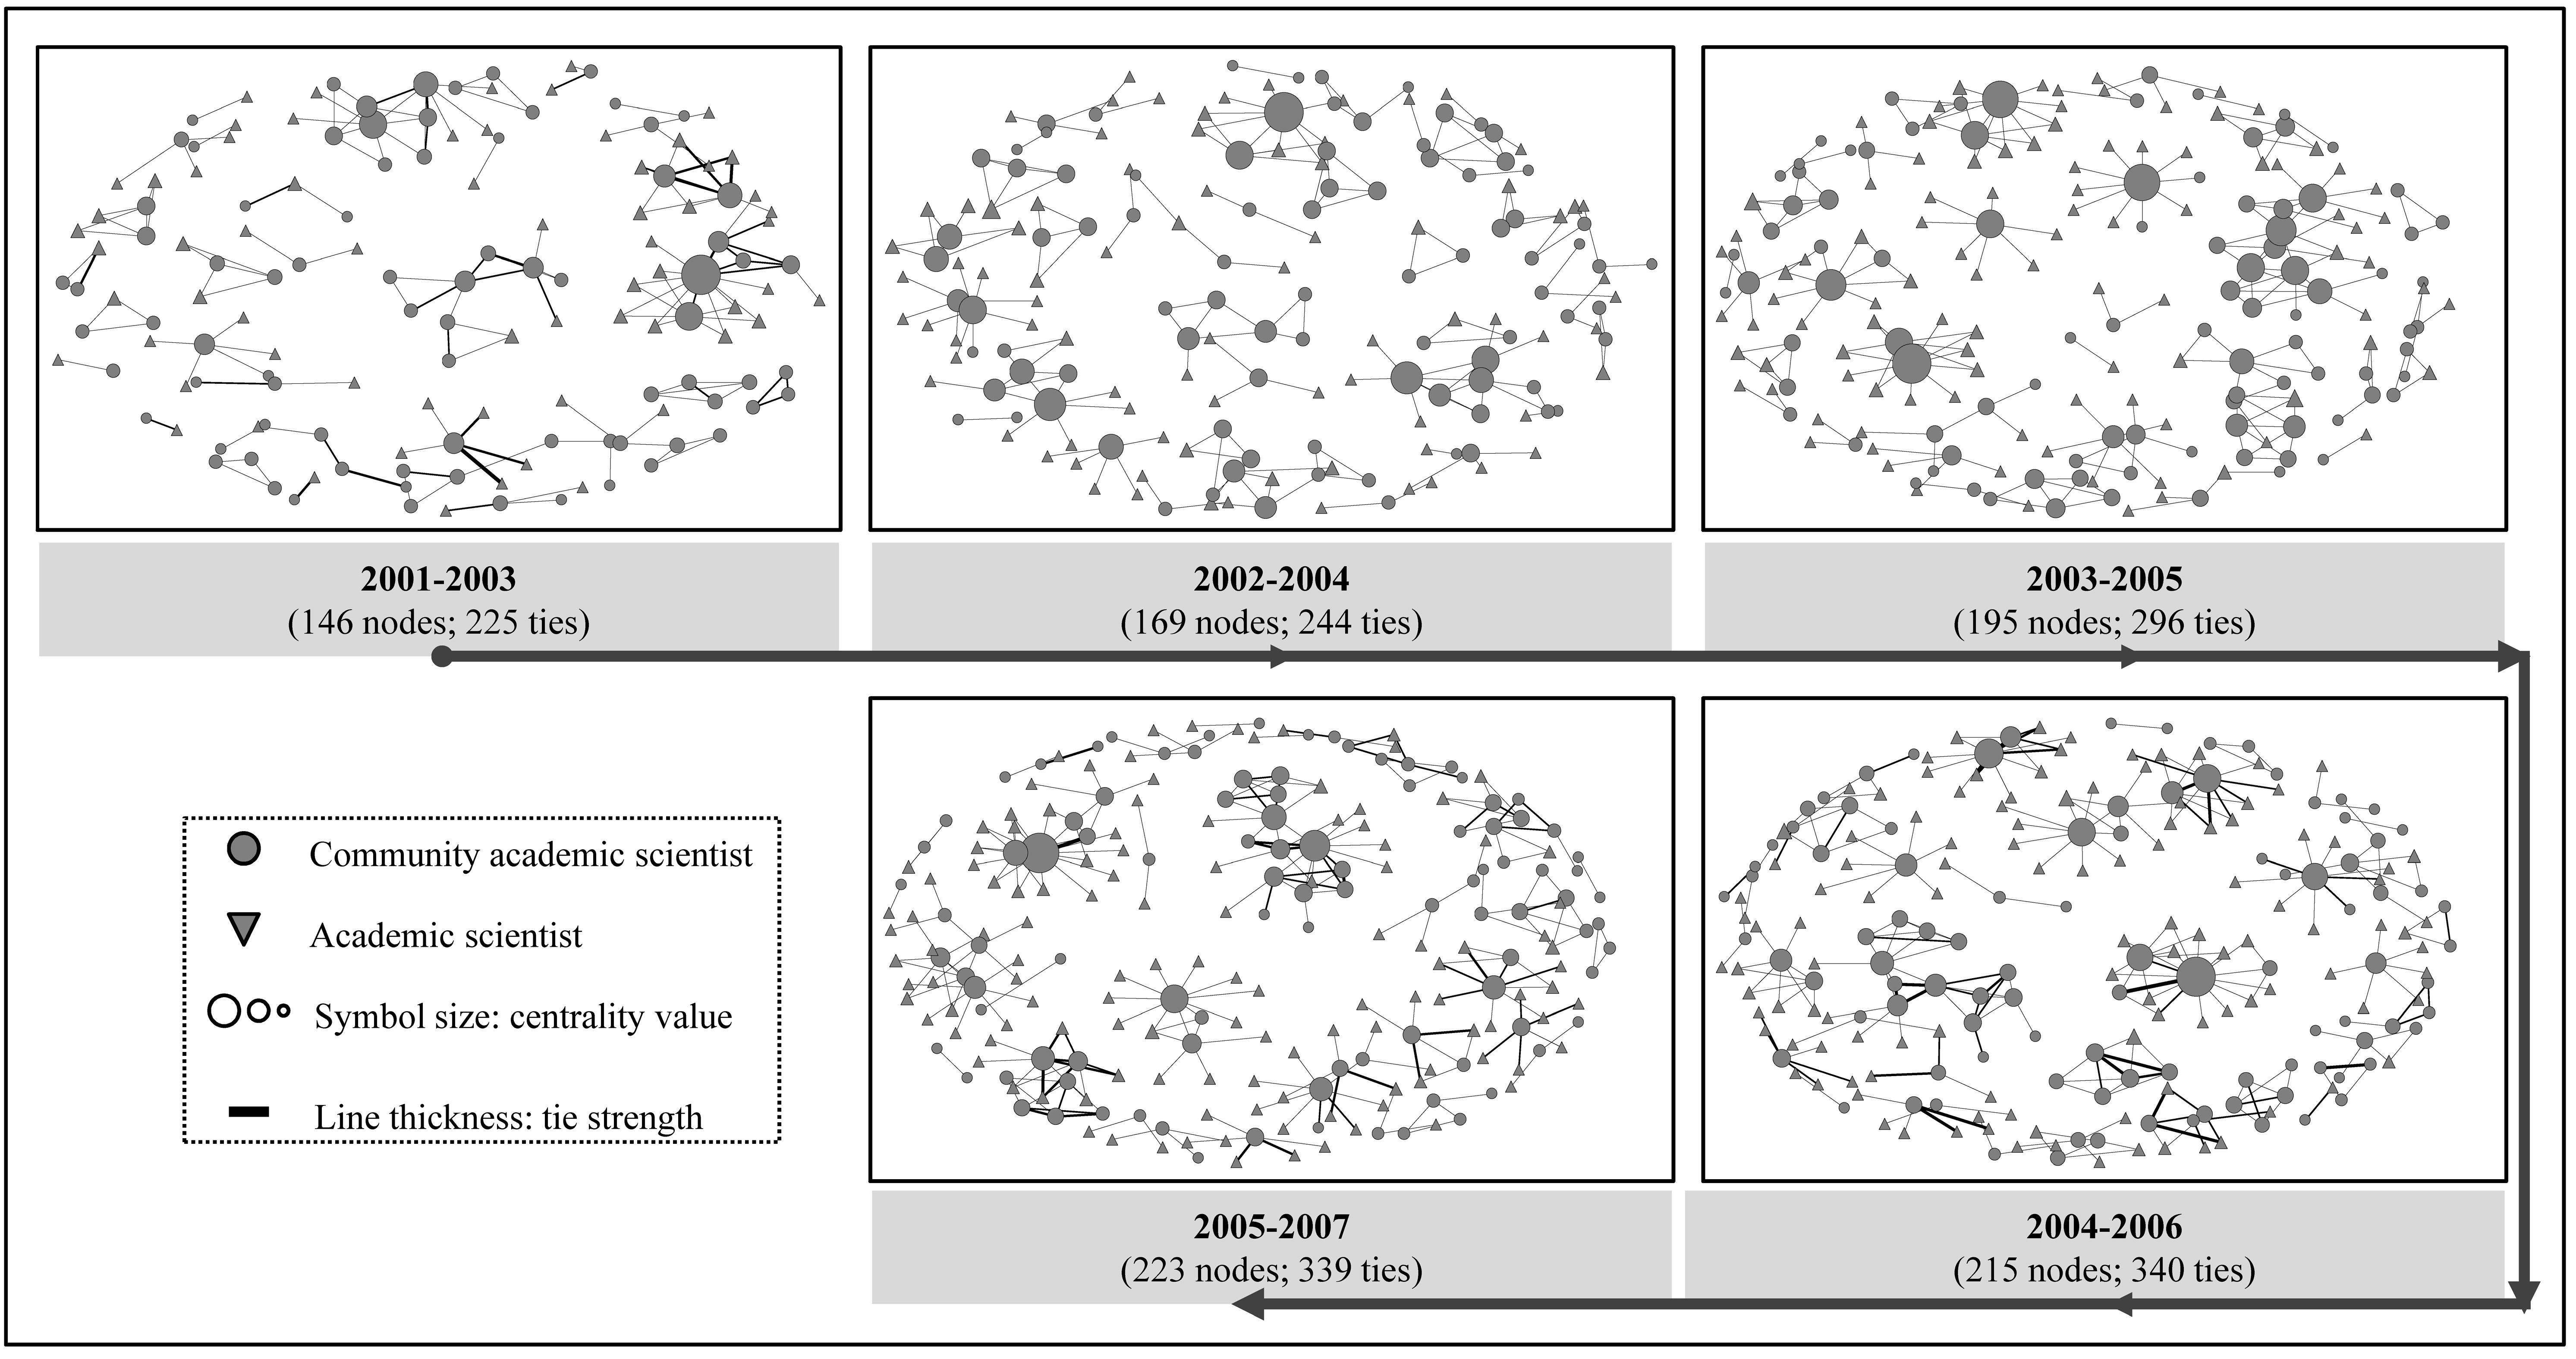
\includegraphics[width=11cm]{job1}\\
\tiny Source: \cite{Rotolo2013}
\end{frame}

%------------------------------------------------

\begin{frame}
\frametitle{\insertsection}
\framesubtitle{Bonacich's centrality (example)}

\centering  
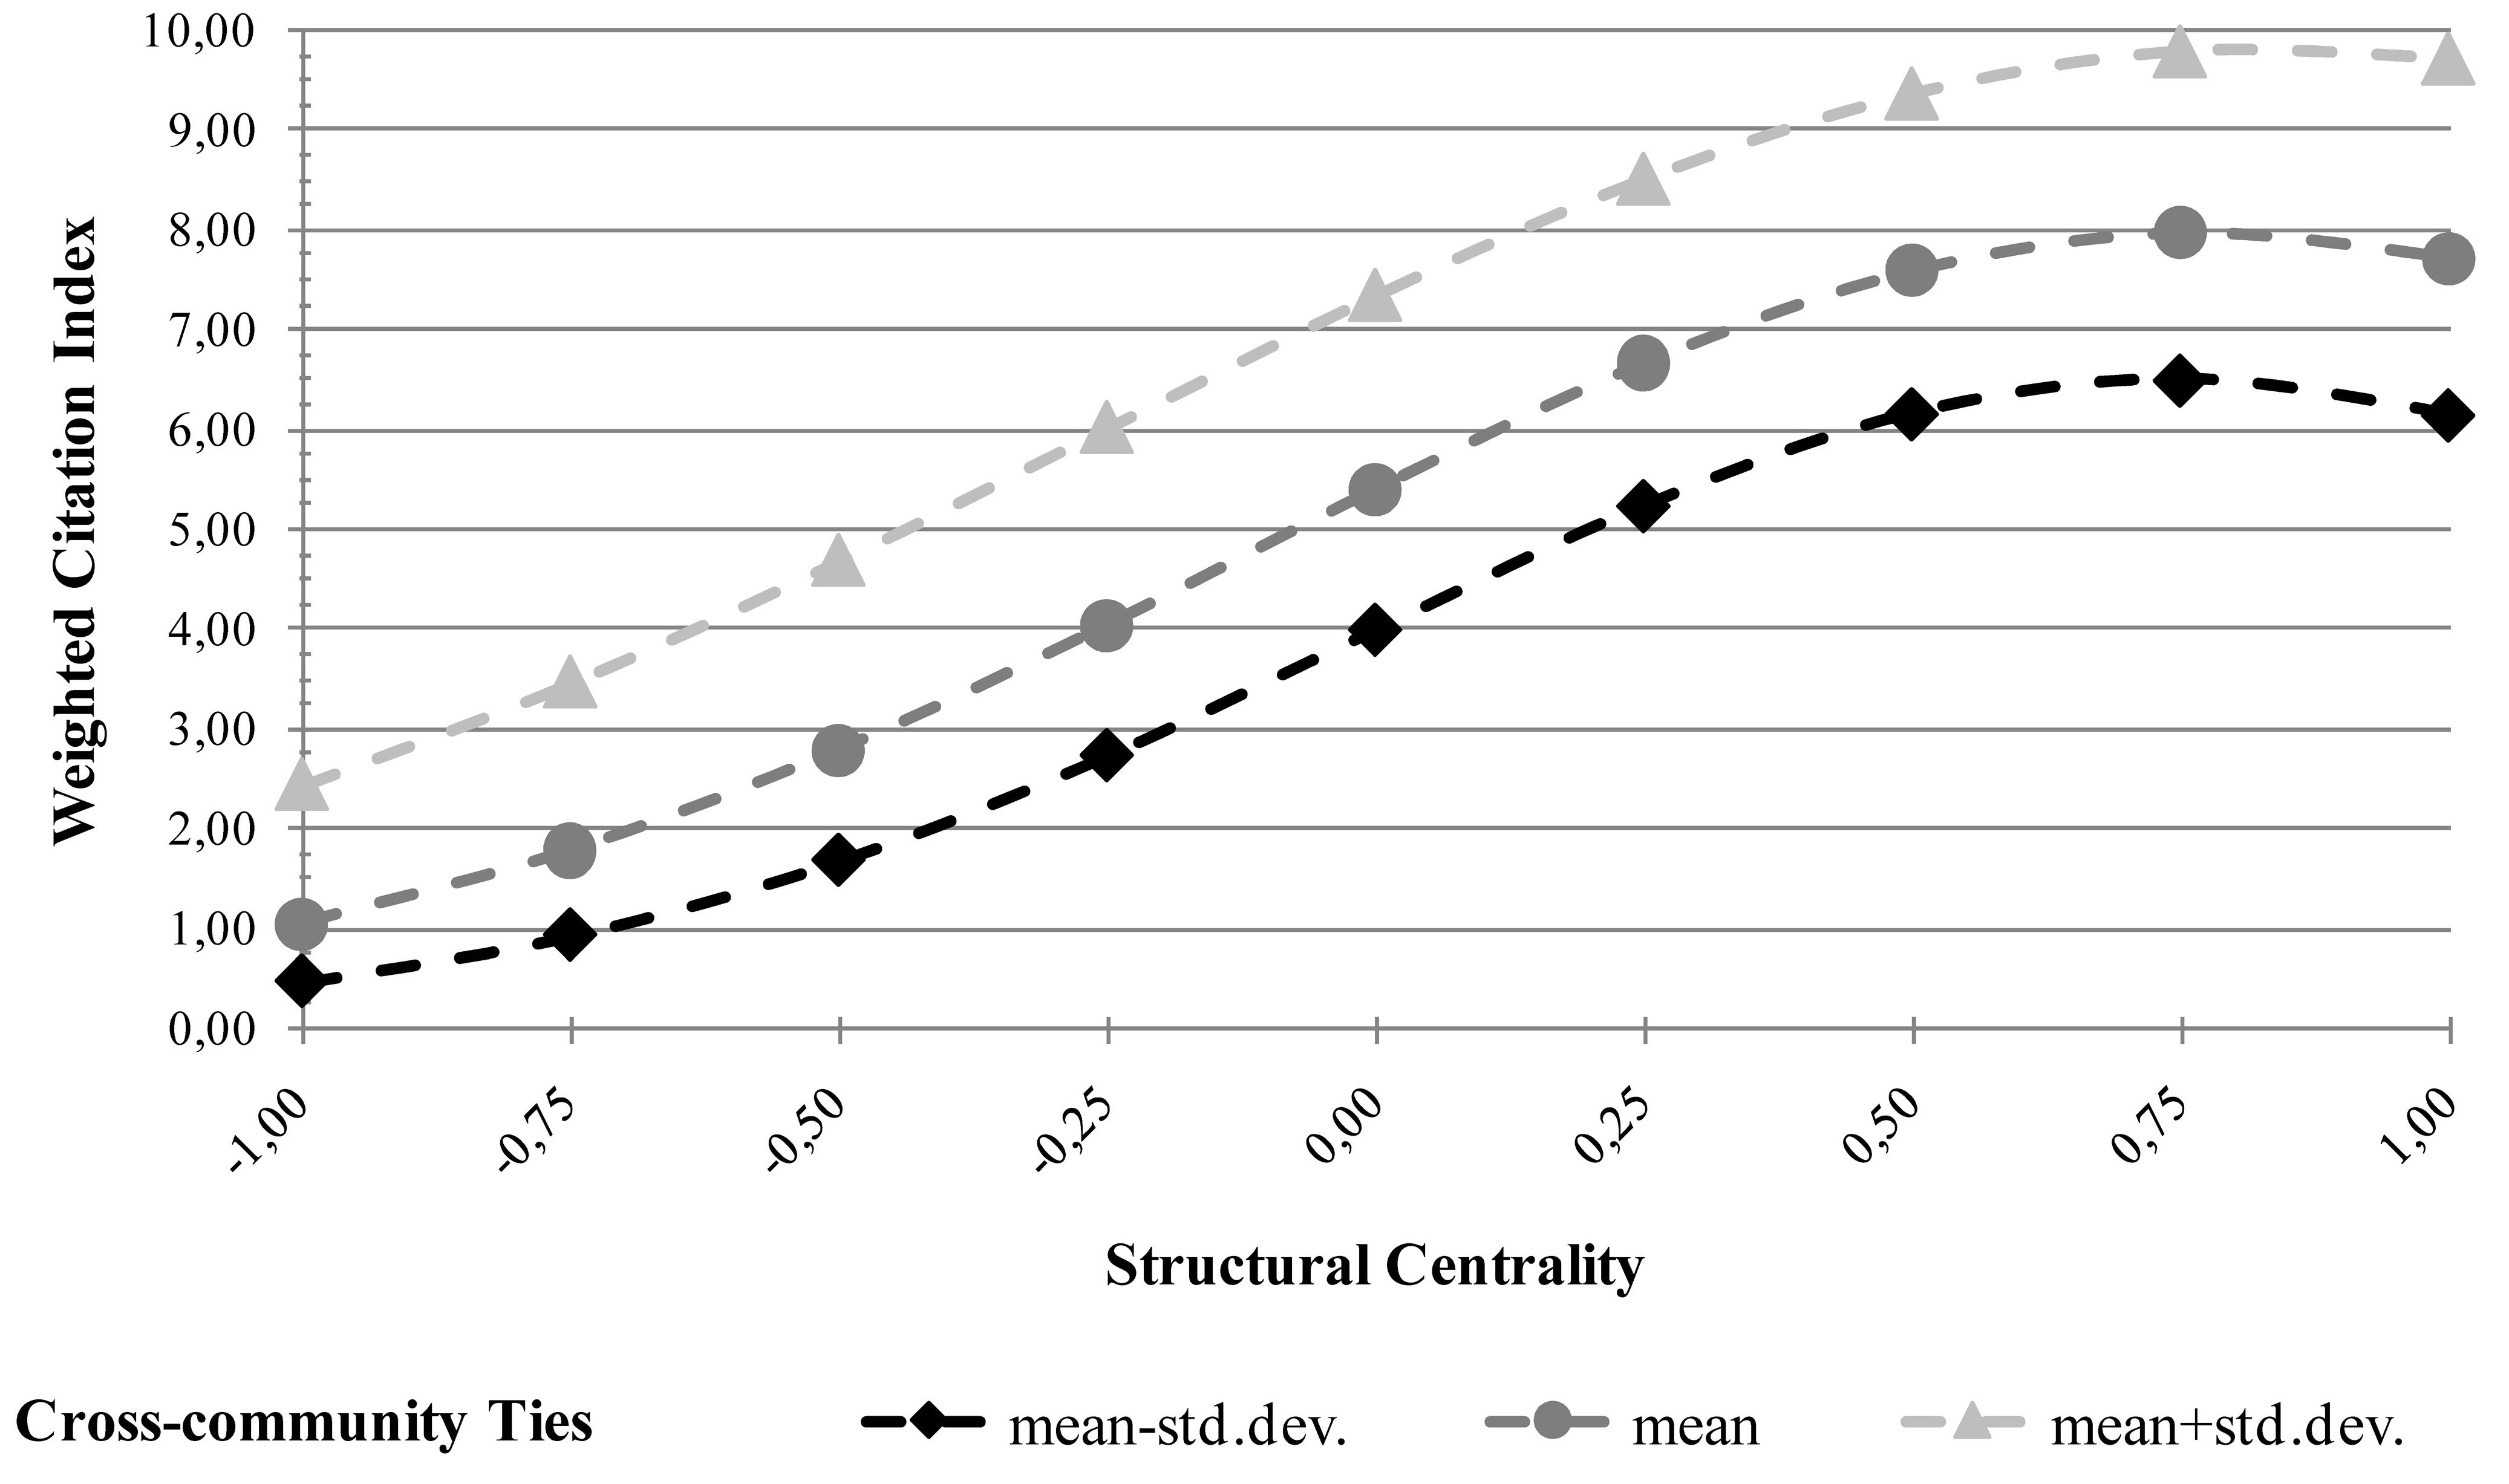
\includegraphics[width= 0.45\textwidth]{job2}\\
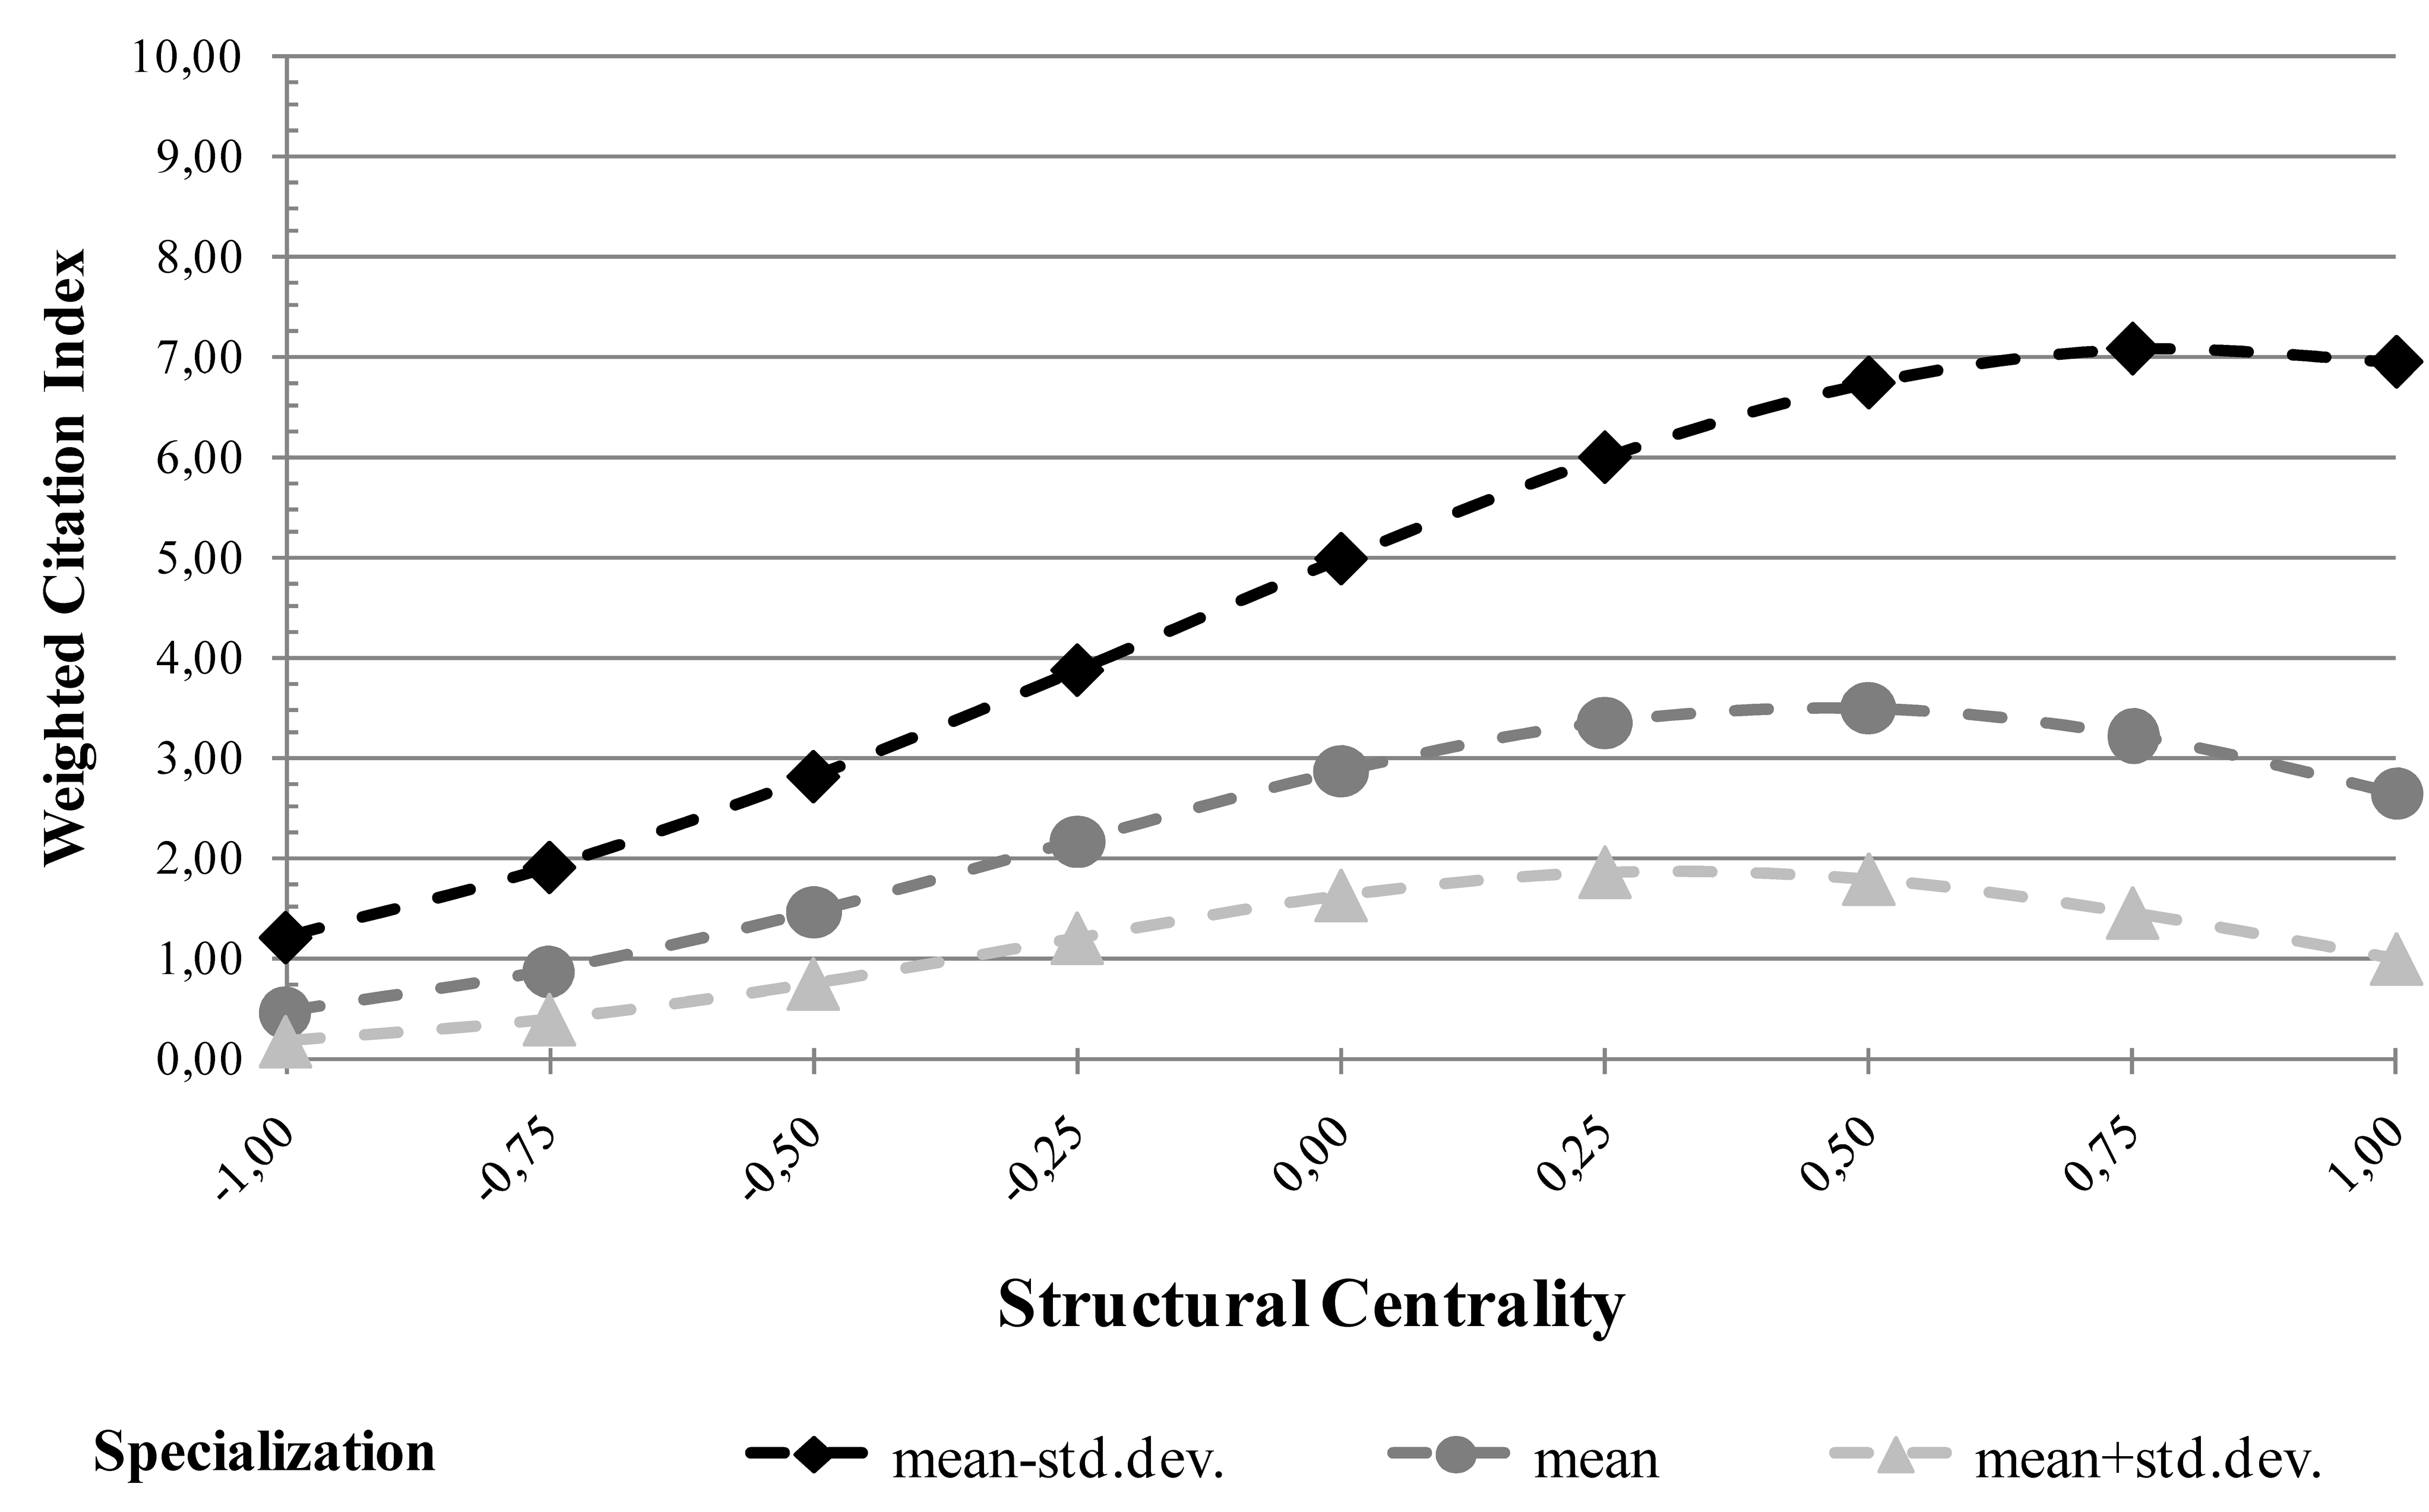
\includegraphics[width= 0.45\textwidth]{job3}\\
\tiny Source: \cite{Rotolo2013}
\end{frame}

%------------------------------------------------


%------------------------------------------------
\subsection{Weighted centrality}
%------------------------------------------------

\begin{frame}
\frametitle{\insertsection}
\framesubtitle{Weighted centrality measures}

\begin{itemize}
	\item The information about the {\color{blue}{strength of ties}} may be provide additional information about the characteristics of the relationships between nodes
	\item {\color{blue}{Social networks}}
		\begin{itemize}
		\item duration/intensity of the relationship
		\item trust
		\item exchange of knowledge
		\item ...
		\end{itemize}
	\item {\color{blue}{Non-social networks}}
		\begin{itemize}
		\item number of goods/people moving between locations
		\item number of synapsis in a neural network
		\item citations between scientific journals
		\item ...
		\end{itemize}
\end{itemize}

\end{frame}

%------------------------------------------------

\begin{frame}
\frametitle{\insertsection}
\framesubtitle{Weighted degree centrality}

\scriptsize
\begin{table}
\begin{tabular}{p{2cm}p{6.5cm}p{2cm}}
\toprule
\textbf{Measure} & \textbf{Defintion} & \textbf{Observation}\\
\midrule
Weighted \newline degree\newline\cite{Barrat2004} & 
$C_D^w(n_i) = \sum_{j=1, i \neq j}^{N-1}{w_{ij}}$\newline
\newline
\newline
- $w_{ij}$, weight of the tie between $n_i$ and $n_j$& 
Number of ties is not considered\\
\\
\hline
\\
Weighted \newline degree\newline\cite{Opsahl2010} & 
$C_D^{w\alpha}(n_i) = C_D(n_i)^{(1-\alpha)}C_D^w(n_i)^\alpha$\newline
\newline
\newline
- $0<\alpha<1$, more importance to degree\newline
- $\alpha=1$, $C_D^w(n_i)$\newline
- $\alpha>1$, less importance to degree&
Number of ties and their weight are both considered\\
\bottomrule
\end{tabular}
\end{table}

\end{frame}

%------------------------------------------------

\begin{frame}
\frametitle{\insertsection}
\framesubtitle{Weighted degree centrality}

\centering  
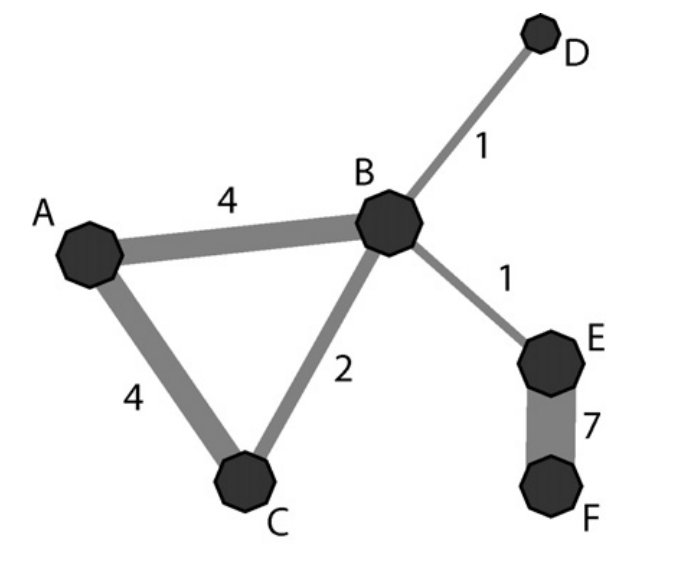
\includegraphics[width=4cm]{degreew2.png}\\
\medskip
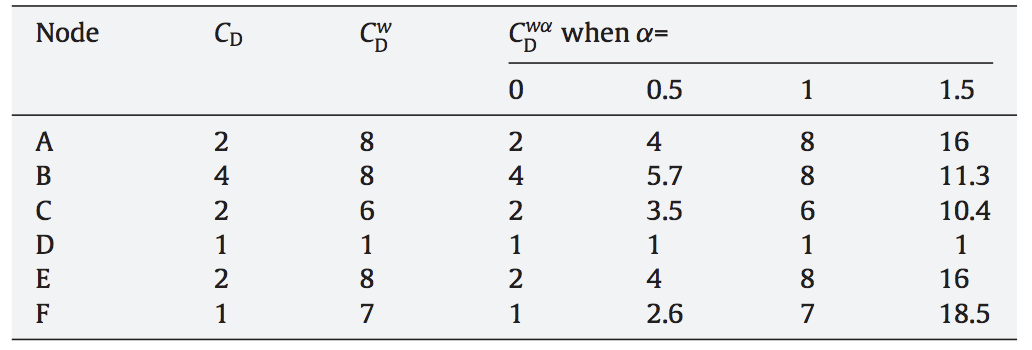
\includegraphics[width=7cm]{degreew1.png}\\
\tiny Source: \cite{Opsahl2010}	

\end{frame}

%------------------------------------------------

\begin{frame}
\frametitle{\insertsection}
\framesubtitle{Weighted closeness centrality}

\scriptsize
\begin{table}
\begin{tabular}{p{2cm}p{6.5cm}p{2cm}}
\toprule
\textbf{Measure} & \textbf{Defintion} & \textbf{Observation}\\
\midrule
Weighted \newline closeness\newline\cite{Newman2001b}&
$C_C^w(n_i) = \left[\sum_{j=1, i \neq j}^{N-1} d^w(n_i, n_j)\right]^{-1}$\newline
\newline
\newline
- $d^w(n_i, n_j) = min(w_{ih}^{-1}+ ... + w_{hj}^{-1})$&
Number of intermediary nodes is not considered\\
\\
\hline
\\
Weighted \newline closeness\newline\cite{Opsahl2010} & 
$C_C^{w\alpha}(n_i) = \left[\sum_{j=1, i \neq j}^{N-1} d^{w\alpha}(n_i, n_j)\right]^{-1}$\newline
\newline
\newline
- $d^{w\alpha}(n_i, n_j) = min(w_{ih}^{-\alpha}+ ... + w_{hj}^{-\alpha})$\newline
- $\alpha=0$, unweighted closeness\newline
- $\alpha=1$, weighted closeness by \cite{Newman2001b}\newline
- $0<\alpha<1$, shortest distance depending on number of nodes\newline
- $\alpha>1$, shortest distance depending on the weight of the ties&
Number of intermediary nodes and their weight are both considered\\
\bottomrule
\end{tabular}
\end{table}

\end{frame}

%------------------------------------------------

\begin{frame}
\frametitle{\insertsection}
\framesubtitle{Weighted closeness centrality}

\centering  
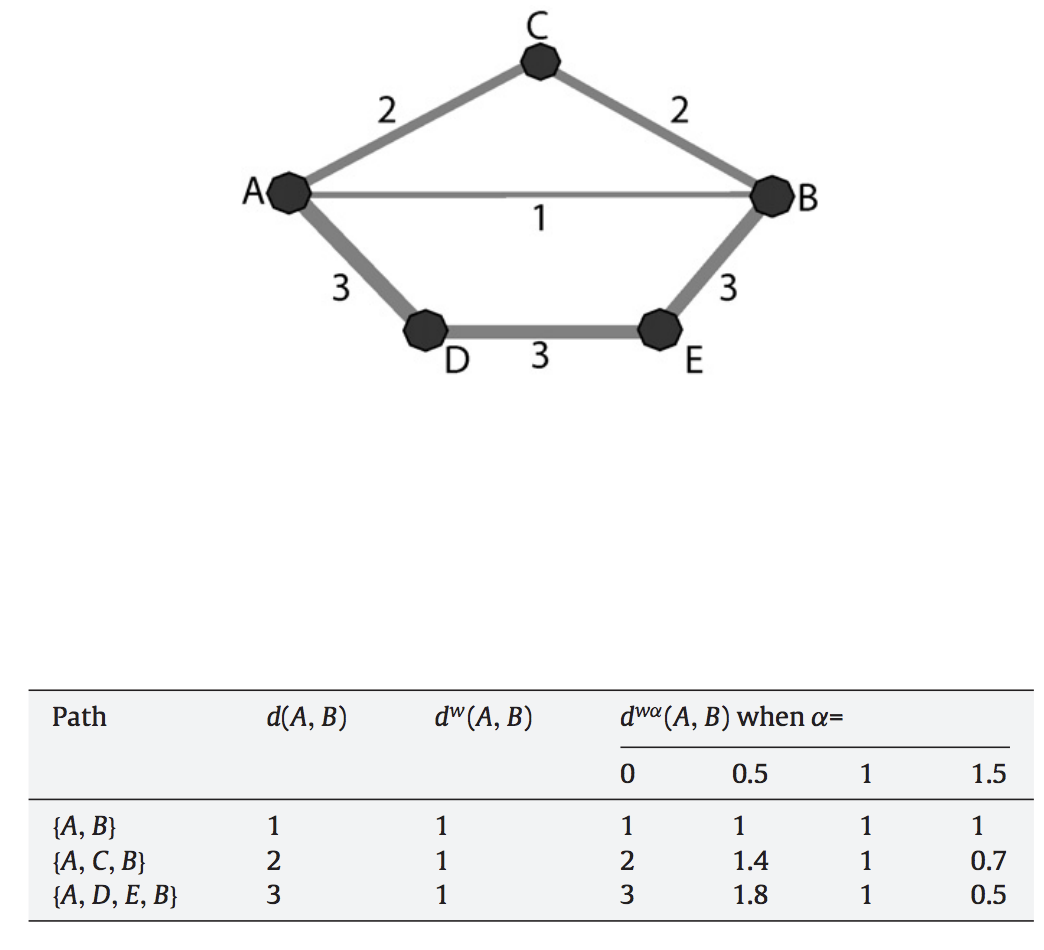
\includegraphics[width=7cm]{distancew.png}\\
\tiny Source: \cite{Opsahl2010}	

\end{frame}

%------------------------------------------------

\begin{frame}
\frametitle{\insertsection}
\framesubtitle{Weighted betweenness centrality	}
\scriptsize
\begin{table}
\begin{tabular}{p{2cm}p{6.5cm}p{2cm}}
\toprule
\textbf{Measure} & \textbf{Defintion} & \textbf{Observation}\\
\midrule
Weighted \newline betweenness\newline\cite{Brandes2008}&
$C_B^w(n_i) = \sum_{j<k \text{ and } j,k \neq i}g_{jk}^w(n_i)/g_{jk}^w$\newline
\newline
\newline
- $g_{jk}^w(n_i)$ shortest paths between nodes $n_j$ and $k$ with $n_i$ \newline
- $d^w(n_i, n_j) = min(w_{ih}^{-1}+ ... + w_{hj}^{-1})$&
Number of intermediary nodes is not considered\\
\\
\hline
\\
Weighted \newline betweenness\newline\cite{Opsahl2010} & 
$C_B^{w\alpha}(n_i) = \sum_{j<k \text{ and } j,k \neq i}g_{jk}^{w\alpha}(n_i)/g_{jk}^{w\alpha}$\newline
\newline
\newline
- $g_{jk}^{w\alpha}(n_i)$ shortest paths between nodes $n_j$ and $k$ with $n_i$ \newline
- $d^{w\alpha}(n_i, n_j) = min(w_{ih}^{-\alpha}+ ... + w_{hj}^{-\alpha})$\newline
- $\alpha=0$, unweighted betweenness\newline
- $\alpha=1$, weighted betweenness by \cite{Brandes2008}\newline
- $0<\alpha<1$, shortest distance depending on number of nodes\newline
- $\alpha>1$, shortest distance depending on the weight of the ties&
Number of intermediary nodes and their weight are both considered\\
\bottomrule
\end{tabular}
\end{table}

\end{frame}

%------------------------------------------------

\begin{frame}
\frametitle{\insertsection}
\framesubtitle{\insertsubsection}

\small
\begin{table}
\begin{tabular}{p{3cm}p{7.5cm}}
\toprule
\textbf{Centrality measure} 	&	\textbf{Interpretation} \\
\hline
\\
Degree 		&	How many nodes can a node reach directly?\\
			&	\textit{\color{blue}information flow, popularity, influence}\\
\\
Closeness        &	    How fast can a node reach every node in the network?\\
			&	\textit{\color{blue}speed, diffusion, efficiency}\\
\\
Betweenness        &	How likely is a node to be part of the most direct route between two nodes in the network?\\
			&	\textit{\color{blue}control, fragmentation, brokerage}\\
\\
Bonacich's centrality 	&	How well is an actor connected to other well-connected actors in the network?\\ 
			&	\textit{\color{blue}power, comprehensive view of the network}\\
\\
Weighted centrality     & Use of the information about the strength of the ties (and distribution of these in the case of Opsahl's centrality)\\
\bottomrule
\end{tabular}
\end{table}
\end{frame}

%------------------------------------------------ 

\begin{frame}
\frametitle{\insertsection}
\framesubtitle{Centrality measures}

\centering  
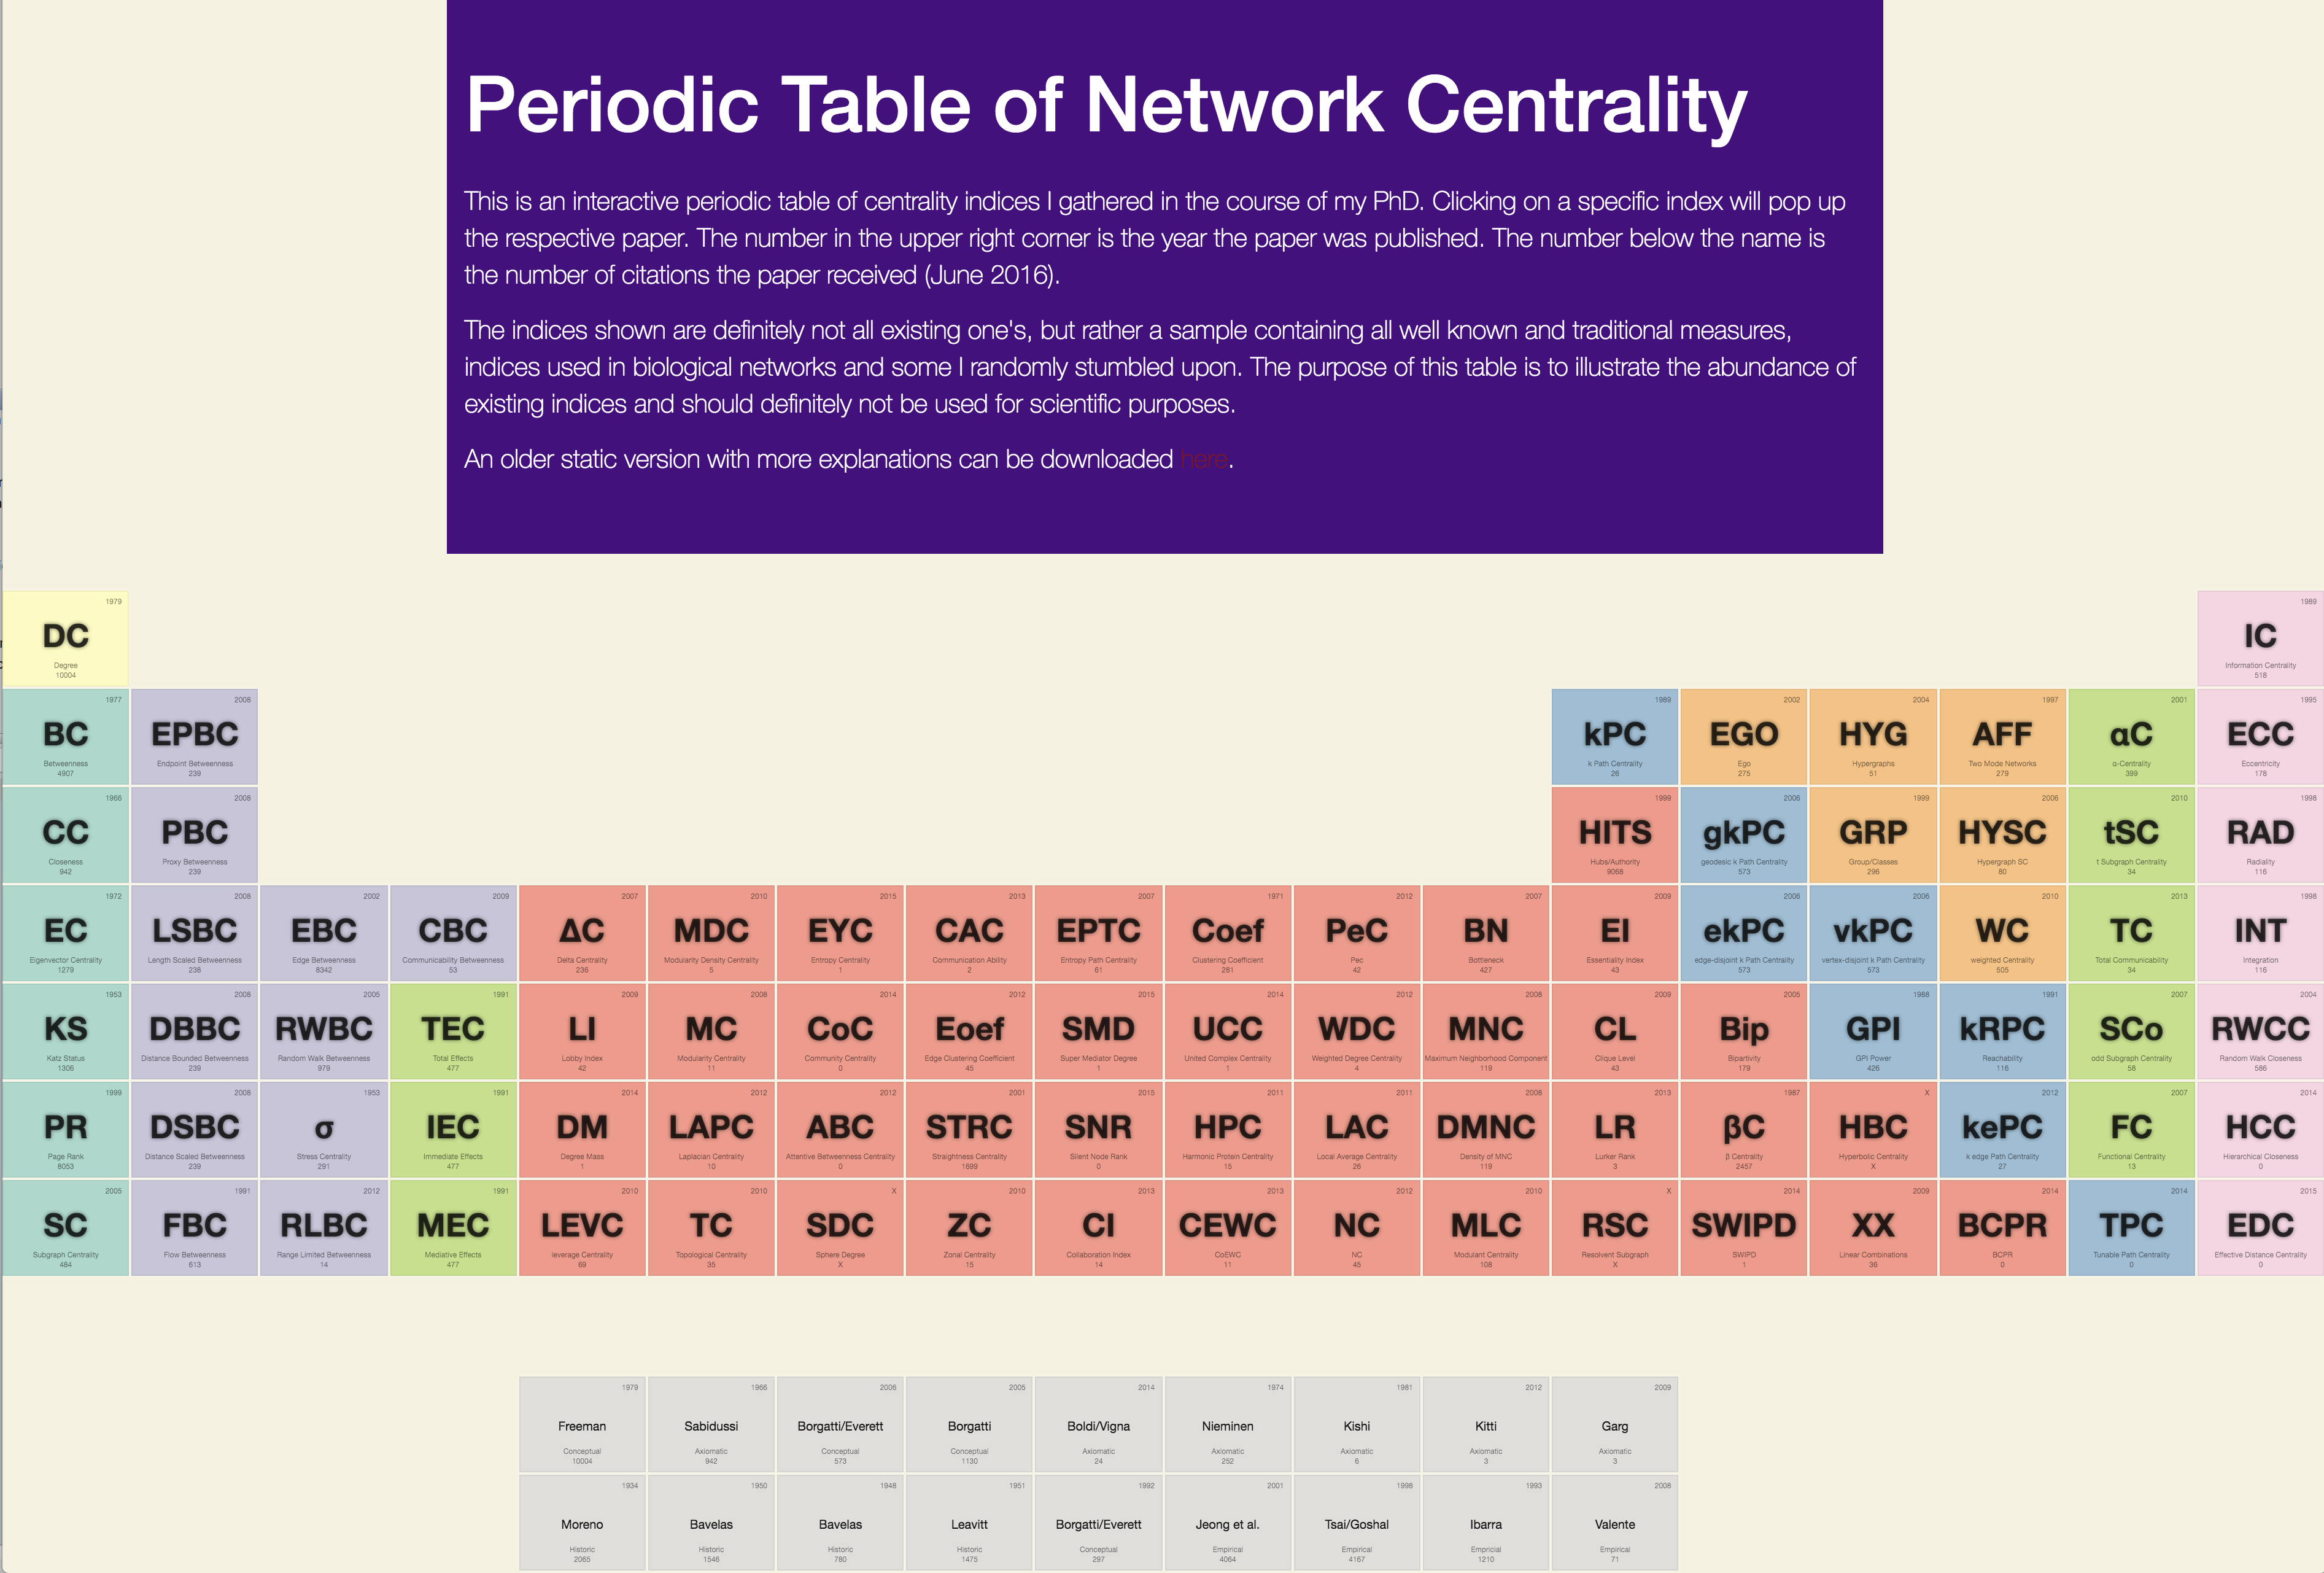
\includegraphics[width=11cm, frame]{periodic}\\
\tiny Source: \url{http://www.schochastics.net/sna/periodic.html}

\end{frame}

%------------------------------------------------



%=======================================================
%	Questions
%=======================================================
\bgroup
\setbeamercolor{background canvas}{bg = orange}
\begin{frame}[plain]{}
\begin{center}
\color{white}{\Huge Questions}
\end{center}
\end{frame}
\egroup
  





%=======================================================
%	Next time ...
%=======================================================
\section*{Next time ...}

%------------------------------------------------

\bgroup
\setbeamercolor{background canvas}{bg = navyblue}
\begin{frame}[plain]{}
\begin{center}
\color{white}{\Huge\insertsection}
\end{center}
\end{frame}
\egroup

%------------------------------------------------

\begin{frame}
\frametitle{\insertsection}

\begin{itemize}

\item 	\textbf{Seminar: Descriptive network analysis B}
	\begin{itemize}
	\item Assessment of node-level measures (centrality measures)
	\end{itemize}
	

\medskip
\medskip

\item 	\textbf{Lecture: Descriptive network analysis C}
	\begin{itemize}
	\item Node-level measures (brokerage measures)
	\end{itemize}

	

		
\end{itemize}

\end{frame}

%------------------------------------------------








%=======================================================
%	References
%=======================================================
\begin{frame}[allowframebreaks]
\frametitle{References}
\tiny
\bibliographystyle{apalike}
\bibliography{references(2).bib}
\end{frame}
%------------------------------------------------




\end{document}